%%%%%%%%%%%%%%%%%%%%%%%%%%%%%%%%%%%%%%%%%%%%%%%%%%%%%%%%%%%
%% Congratulations, you've made an excellent choice
%% of writing your Tampere University thesis using
%% the LaTeX system. This document attempts to be
%% as complete a template as possible to let you focus
%% on the most important part: the writing itself.
%% Thus the details regarding the visual appearance
%% and even structure have already been worked out
%% for you!
%%
%% I sincerely hope you will find this template useful
%% in completing your thesis project. I've tried to
%% add comments (followed by the % sign) to clarify
%% the structure and purpose of some of the commands.
%% Most of the magic happens in the file tauthesis.cls,
%% which you are more than welcome to take a look at.
%% Just refrain from editing it in the most crucial
%% versions of the thesis!
%%
%% I wish you and your thesis project the best of luck!
%% If this template causes you trouble along the way
%% or if you've any suggestions for improving it,
%% please be in contact through GitHub
%% (<URL HERE>)
%%
%% Yours,
%%
%% Ville Koljonen
%%
%% PS. This template or its associated class file don't
%% come with a warranty. The content is provided as is,
%% without even the implied promise of fitness to the
%% mentioned purpose. You, as the author of the thesis,
%% are responsible for the entire work, including the
%% provided material. No one else is liable to you for
%% any damage inflicted on you or your thesis, were it
%% caused by using this template or not.
%%%%%%%%%%%%%%%%%%%%%%%%%%%%%%%%%%%%%%%%%%%%%%%%%%%%%%%%%%%

%%%%% NOTICE %%%%%
%% Please read through the entire template
%% (files under ./tex) to find all instructions.
%% It is possible that the attached pdf files
%% do not include the latest information.
%%%%%%%%%%%%%%%%%%

%%%%% INSTRUCTIONS FOR COMPILING THE DOCUMENT %%%%%
%% Overleaf: just click Recompile.
%% Terminal:
%%  1. pdflatex main.tex
%%  2. makeindex -s main.ist -t main.glg -o main.gls main.glo
%%  3. biber main
%%  4. pdflatex main.tex
%%  5. pdflatex main.tex
%% Similar sequence of commands is also required
%% in LaTeX specific editors.
%%%%%%%%%%%%%%%%%%%%%%%%%%%%%%%%%%%%%%%%%%%%%%%%%%%

%%%%% METADATA %%%%%
%
% Always keep the following metadata up to date! This is important for your
% PDF file to comply to accessibility standards. (And yes, this information
% must remain here, before \documentclass[...]{...}.)

%
% metadata.tex
%
% Fill in your document metadata in this file.
% This is included into the file main.tex for you.
%


\def\myfititle{Kuvaava otsikko}
\def\myentitle{A Descriptive title}
\def\myauthor{Firstname Lastname}
\def\myfisubtitle{Tarkentava alaotsikko}
\def\myensubtitle{A Specifying Subtitle}
\def\myfithesistype{Opinnäytetyön taso}
\def\myenthesistype{Thesis type}
\def\myexaminers{Title1 Firstname1 Lastname1 \\ Title2 Firstname2 Lastname2 \\ ...}
\def\myfifacultyname{Tiedekunnan nimi}
\def\myenfacultyname{The name of the faculty}
\def\myfiprogrammename{Tutkinto-ohjelman nimi}
\def\myenprogrammename{The name of the study programme}
\def\myfikeywords{avainsana1, avainsana2, ...}
\def\myenkeywords{keyword1, keyword2, ...}
\def\mylanguagecode{en-US}
\def\mysubject{A short description of the thesis subject.}
\def\myyear{2023}
\def\mymonth{06}
\def\myday{03}

% Define your citation options here.
% Valid values for style and sorting options
% can be found in the BibLaTeX manual: https://ctan.org/pkg/biblatex.

\def\mycitationstyle{numeric}
\def\mycitationsorting{nyt}


\input{preamble.tex} % You can add packages and define new commands in this file.

\begin{document}

%%%%% FRONT MATTER %%%%%

%%%%% Thesis information and title page.

\titlepagematter

\maketitle

\frontmatter



\serialNumberPage

%%%%% Abstracts and preface.
%
% Write the abstract(s) and the preface into a separate file for the sake of
% clarity. Pass the appropriate file name as the first argument to these
% commands. Put the \abstract in the primary language first and the
% \otherabstract in the secondary language second. Those who do not speak
% Finnish only need the first abstract. The second argument of the \preface
% command takes the place where the thesis was signed in.
%
% Edit the files tex/{use-of-ai-en, use-of-ai-fi}.tex to match your use of AI in
% generating this thesis.
%

\abstract

\otherabstract

\preface{Tampere}

%%%%% Table of contents.


\hypersetup{
	linkcolor=black,
}

\tableOfContents

%%%%% Lists of figures, tables, listings and terms.
%
% Print the lists of figures and/or tables. Uncomment either of these commands
% as required. Both are optional, but if there are many important
% figures/tables, listing them may be a good idea.

\listOfFigures

\listOfTables

\listOfListings

% Misc stuff related to how the glossary is displayed.

\glsaddall
\setglossarystyle{taulong}
\setlength{\glsnamewidth}{0.25\textwidth}
\setlength{\glsdescwidth}{0.75\textwidth}
\renewcommand*{\glsgroupskip}{}

% Print the default glossary of abbreviations, if necessary. Otherwise comment
% out. The appropriate Finnish variant is 'Lyhenteet'

\printglossary[type=main]

% Print more than one glossary with these lines. Otherwise comment out.

% \printglossary[type=symbs]
% \printglossary[type=label]
% ...

\listofpublications

% AI disclaimer page.

\aidisclaimerinclusioncmd


%%%%% MAIN MATTER %%%%%

\mainmatter

\hypersetup{
	linkcolor=taupurple,
}

% Actually include your chapters in the file specified by this input statement.

%
% index.tex
%
% This file is where you should include your actual content. Write each of
% the chapters of the thesis into a separate file for the sake of clarity.
% They can be \input as shown below. Give both the chapters and their files as
% descriptive names as possible.
%

\chapter{Introduction}
\label{ch:introduction}

This chapter introduces the research topic, providing background information and outlining the motivation behind the study. It also presents the research objectives and questions that guide the investigation.

\section{Background and Motivation}
\label{sec:background-and-motivation}

In recent years, the integration of Artificial Intelligence (AI) assistants into various software systems has gained significant attention. AI assistants have the potential to enhance user experience, streamline workflows, and improve decision-making processes. Product Lifecycle Management (PLM) systems, which manage the entire lifecycle of a product from inception to disposal, can particularly benefit from the integration of AI assistants. By leveraging AI technologies, PLM systems can provide users with intelligent support, automate routine tasks, and facilitate better collaboration among stakeholders.

\section{Research Objectives and Questions}
\label{sec:research-objectives-and-questions}

The primary objective of this research is to develop an AI assistant that is seamlessly integrated with a PLM system, enhancing the overall user experience and improving decision-making processes. To achieve this objective, we have formulated the following research questions:

\begin{itemize}
	\item \textbf{RQ1 (Design)}: What RAG system architecture best fits Sovelia Core's on-prem, PostgreSQL-based environment and data governance constraints?
	\item \textbf{RQ2 (Process)}: How should customer documentation pipelines (parse $ \rightarrow $ chunk $ \rightarrow $ embed $ \rightarrow $ retire) be engineered for reliability and maintainability?
	\item \textbf{RQ3 (Quality \& Risk)}: Which risks (hallucinations, stale context, access control) are most critical, and what mitigations work in practice?
\end{itemize}


\chapter{Literature review}
\label{ch:literature-review}

This chapter establishes the theoretical and empirical foundation and background for integrating a resource-augmented AI assistant into Sovelia Core PLM. The review begins by examining the fundamental characteristics of Product Lifecycle Management systems and the role of AI assistants in data-intensive workflows, establishing why a human-in-the-loop considerable approach for enterprise PLM environments (\autoref{sec:plm-systems-and-ai-assistants}). After this, the overall architecture and principles of Retrieval-Augmented Generation (RAG) systems is explained briefly, focusing on how the combination of parametric and non-parametric memory addresses key limitations of purely parametric models in knowledge-intensive tasks (\autoref{sec:resource-augmented-ai-systems}).

The core of this review examines five recent case studies of RAG-based systems deployed in technical documentation and manufacturing contexts (\autoref{sec:case-studies-on-similar-integrations}): Heredia Álvaro and Barreda's ceramic tile manufacturing quality control system, Shejuti et al.'s technical documentation chatbot, Knollmeyer et al.'s manufacturing documentation system with knowledge graph enhancement, Wan et al.'s hybrid KG-vector RAG for smart manufacturing, and Wang et al.'s comprehensive framework for AI in PLM. These studies reveal both common success factors, particularly in domain-specific adaptation, and persistent challenges. The contexts of these studies are comparable to those of typical PLM system users, who are predominantly in the manufacturing industry \parencite{stark_product_2015}. By synthesizing lessons from these deployments, this review identifies key design considerations and risk factors to inform the architecture and implementation strategy of the AI assistant for Sovelia Core, especially given the challenges faced by companies in the manufacturing industry.

\section{Overview of PLM systems and AI assistants}
\label{sec:plm-systems-and-ai-assistants}

Product Lifecycle Management (PLM) systems are integral to managing the entire lifecycle of a product from inception, through engineering design and manufacturing, to service and disposal. They provide a centralized repository for all product-related information, facilitating collaboration among different departments and stakeholders \parencite{stark_product_2015}. In PLM systems generally the lifecycle states of product include: imagine, define, realise, support/use and retire/dispose \parencite{stark_product_2015-1}. All these separate stages generate data (including documentation) that needs to be managed effectively. The purpose of PLM system is to centralize all this data and provide users with access to the right information at the right time.

AI assistants, in the context of data-intensive workflows, can be defined as \textit{semi-automatic interactive tools} that guide analysts through specific tasks by recommending suitable transformations or actions that respect constraints obtained through interaction with the analyst \parencite{petricek_ai_2023}. Analysts in this context mean the human utilizing the AI assistant. Unlike fully automatic systems that attempt to solve problems without human intervention, or purely manual tools that require complete human control, AI assistants implement an iterative interaction pattern where the system makes an initial recommendation, the user can provide feedback through structured constraints or selections, and the system refines its recommendations accordingly. This human-in-the-loop approach combines the scalability and automation of machine learning with critical human insight, making it particularly suitable for tasks where edge cases and domain-specific knowledge are crucial \parencite{petricek_ai_2023}. In this thesis, the aim is to develop an AI assistant that can be integrated into PLM system to enhance user experience by providing context-aware support, streamlining routine data wrangling tasks, and improving access to information while maintaining human oversight and control. The AI assistant is meant to provide users with answers based on the documentation stored within the PLM system's database. However, the AI assistant in the context of this thesis is not fully automatic, as the users still have control over the final decisions and actions taken based on the AI assistant's recommendations. The purpose of the AI assistant is to inform and help with decision-making, rather than replacing human judgment entirely.

\section{Resource-augmented AI systems}
\label{sec:resource-augmented-ai-systems}

Resource-augmented AI systems, also known as \emph{retrieval-augmented generation} (RAG) systems, represent a paradigm shift in how artificial intelligence systems access and utilize knowledge. Unlike purely parametric models that store all knowledge implicitly within their parameters, resource-augmented systems combine parametric memory (the weights of a neural network) with non-parametric memory (external knowledge sources such as databases, document collections, or knowledge graphs) \parencite{lewis_retrieval-augmented_2021}. This hybrid architecture addresses several fundamental limitations of parametric-only models: the inability to easily update or revise stored knowledge, difficulty in providing provenance for predictions, and the tendency to generate hallucinated or factually incorrect content \parencite{lewis_retrieval-augmented_2021}. In simplified terms, RAG systems can be viewed as AI systems that "look up" relevant information from an external source before generating a response, rather than relying solely on learned patterns from training data and thus enabling more accurate, up-to-date, and contextually relevant outputs. This will result in less hallucinations compared to standard large language models (LLMs) \parencite{lewis_retrieval-augmented_2021}.

\begin{figure}[htbp]
    \centering
    \small{\resizebox{\textwidth}{!}{% generated by Plantuml 1.2025.9       
\definecolor{plantucolor0000}{RGB}{0,0,0}
\definecolor{plantucolor0001}{RGB}{255,255,255}
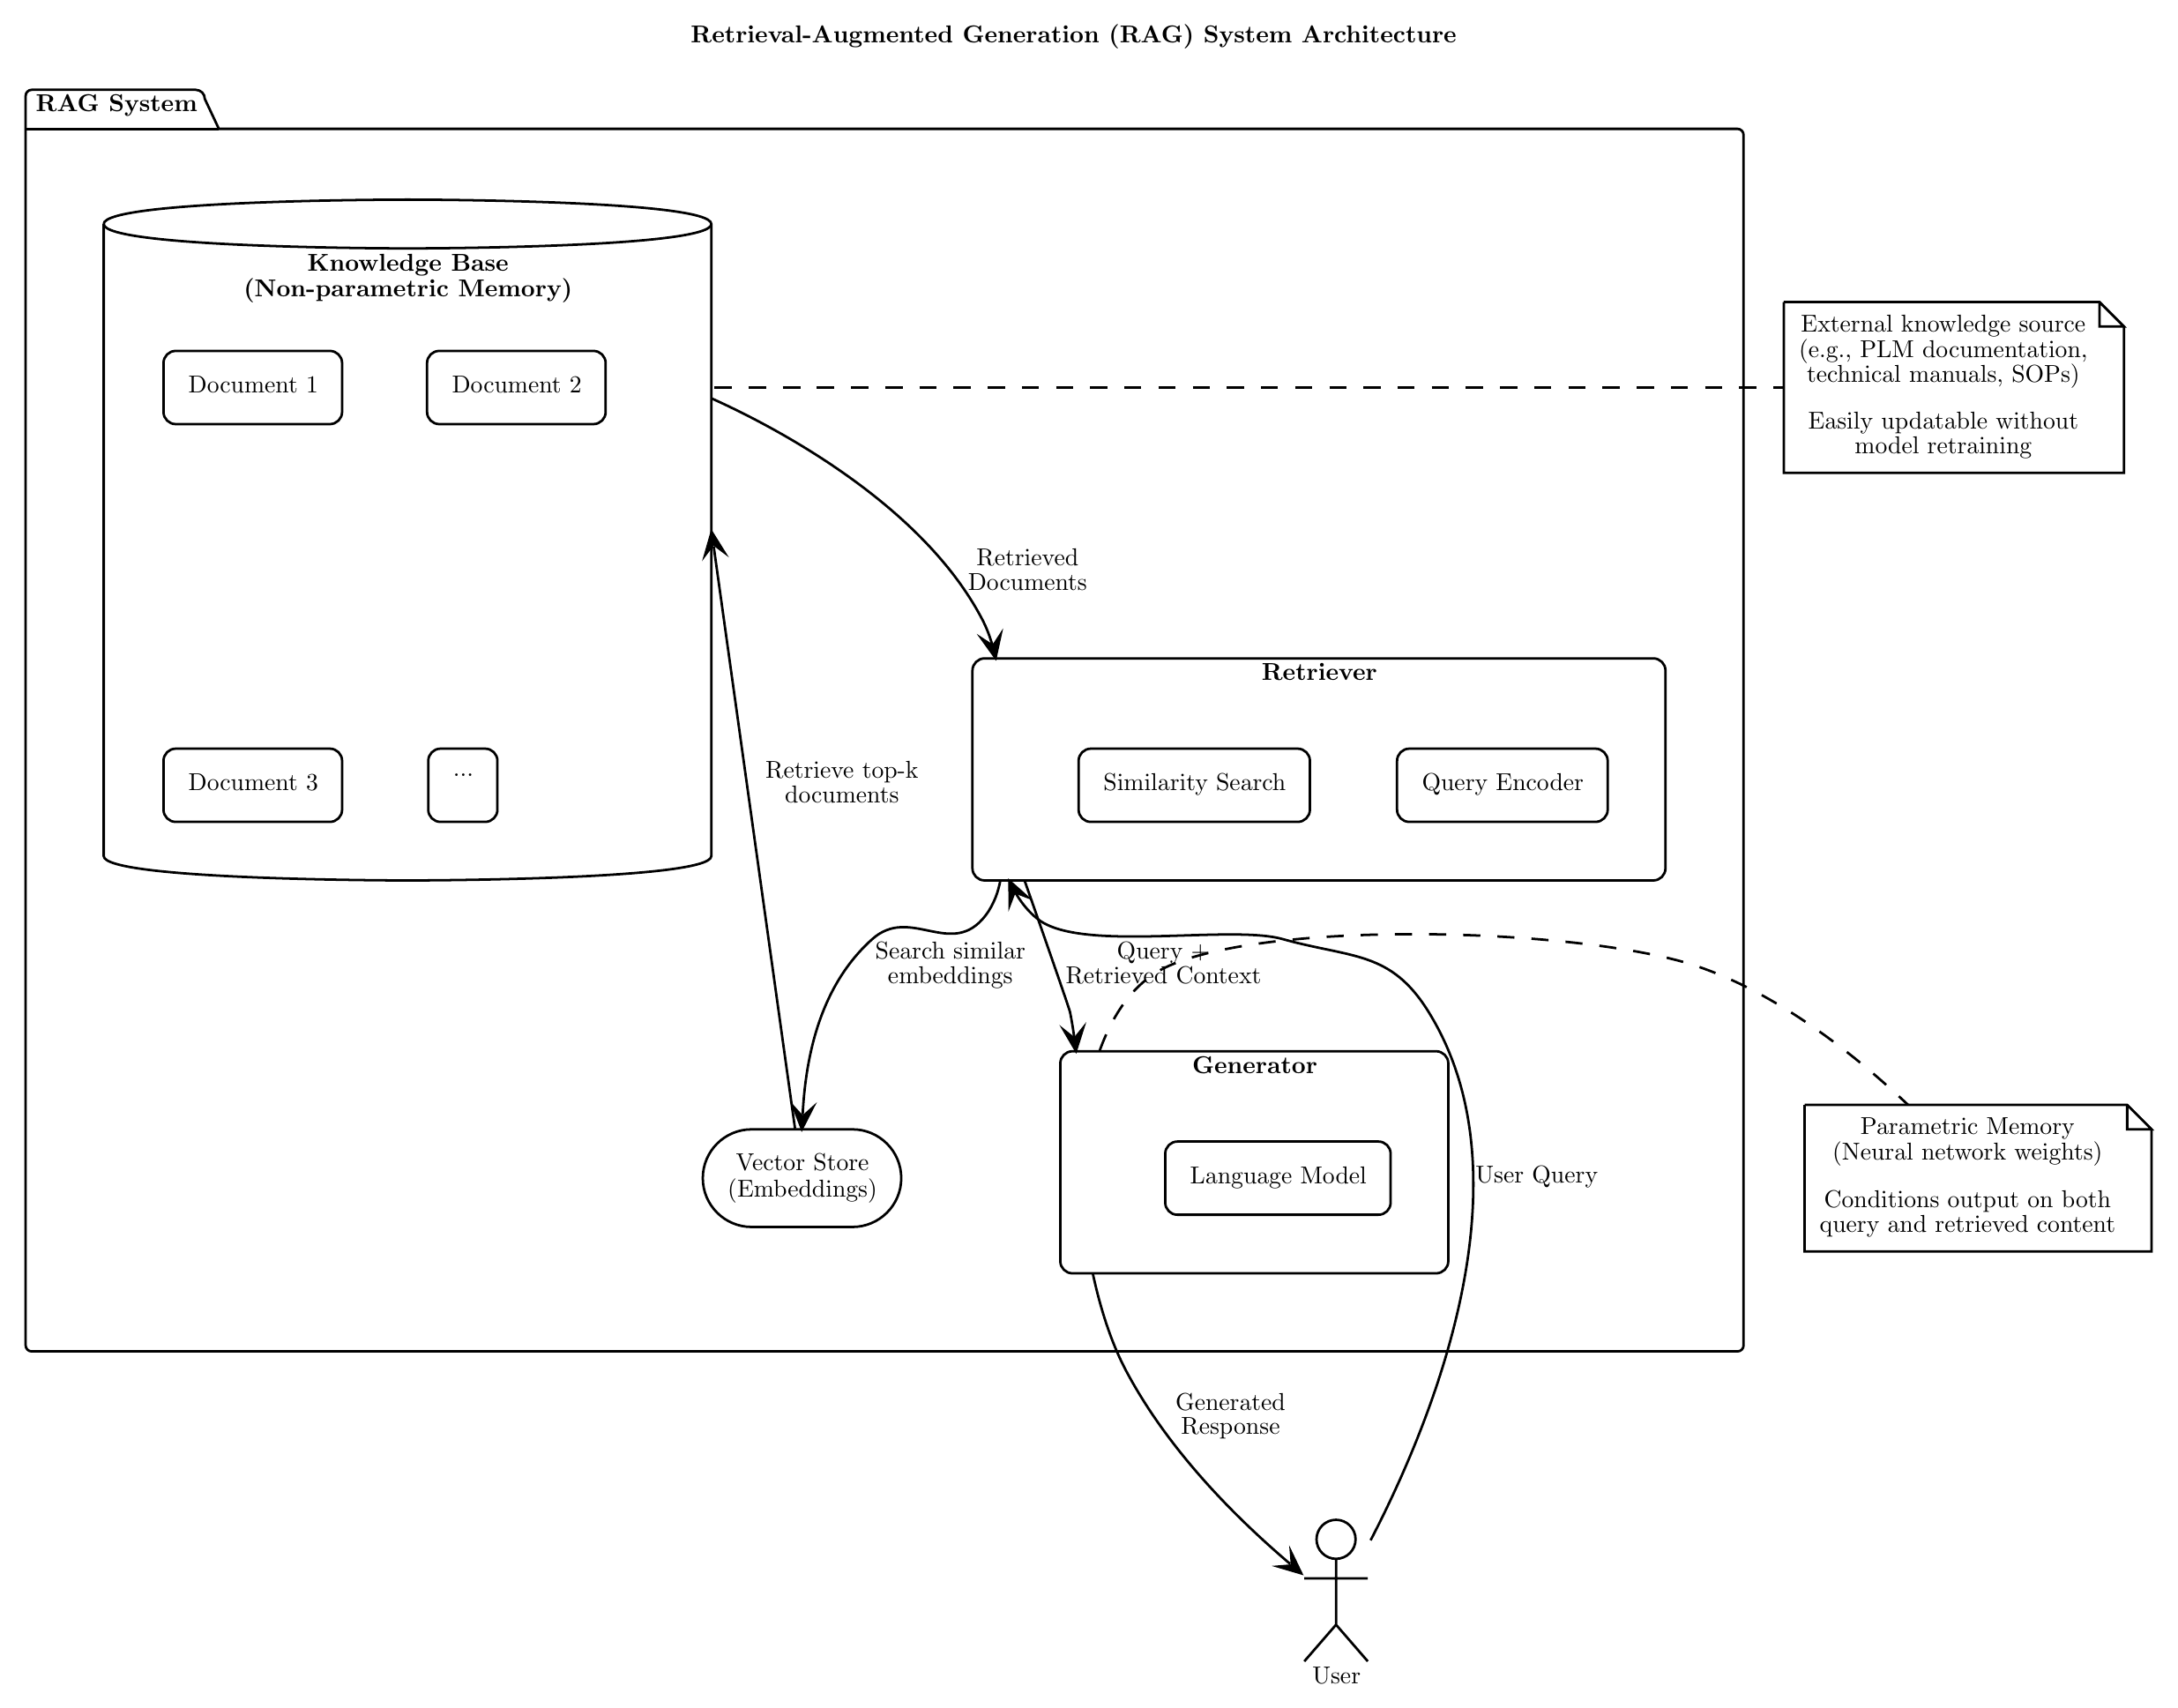
\begin{tikzpicture}[yscale=-1
,pstyle0/.style={color=black,fill=white,line width=1.0pt}
,pstyle1/.style={color=black,line width=1.0pt}
,pstyle2/.style={color=black,fill=black,line width=1.0pt}
,pstyle3/.style={color=black,line width=1.0pt,dash pattern=on 7.0pt off 7.0pt}
]
\node at (283.395pt,15pt)[below right,color=black,inner sep=0]{\textbf{Retrieval-Augmented Generation (RAG) System Architecture}};
\draw[pstyle0] (13.5pt,42pt) -- (80.69pt,42pt) arc(270:360:3.75pt)  -- (90.19pt,58pt) -- (712.5pt,58pt) arc(270:360:2.5pt)  -- (715pt,556.5pt) arc(0:90:2.5pt)  -- (13.5pt,559pt) arc(90:180:2.5pt)  -- (11pt,44.5pt) arc(180:270:2.5pt) ;
\draw[pstyle1] (11pt,58pt) -- (90.19pt,58pt);
\node at (15pt,44pt)[below right,color=black,inner sep=0]{\textbf{RAG System}};
\draw[pstyle0] (399pt,280pt) arc (180:270:5pt) -- (404pt,275pt) -- (678pt,275pt) arc (270:360:5pt) -- (683pt,280pt) -- (683pt,361pt) arc (0:90:5pt) -- (678pt,366pt) -- (404pt,366pt) arc (90:180:5pt) -- (399pt,361pt) -- cycle;
\node at (517.335pt,277pt)[below right,color=black,inner sep=0]{\textbf{Retriever}};
\draw[pstyle0] (435pt,441pt) arc (180:270:5pt) -- (440pt,436pt) -- (589pt,436pt) arc (270:360:5pt) -- (594pt,441pt) -- (594pt,522pt) arc (0:90:5pt) -- (589pt,527pt) -- (440pt,527pt) arc (90:180:5pt) -- (435pt,522pt) -- cycle;
\node at (488.87pt,438pt)[below right,color=black,inner sep=0]{\textbf{Generator}};
\draw[pstyle0] (43pt,97pt) ..controls (43pt,87pt) and (167.5pt,87pt) .. (167.5pt,87pt) ..controls (167.5pt,87pt) and (292pt,87pt) .. (292pt,97pt) -- (292pt,356pt) ..controls (292pt,366pt) and (167.5pt,366pt) .. (167.5pt,366pt) ..controls (167.5pt,366pt) and (43pt,366pt) .. (43pt,356pt) -- (43pt,97pt);
\draw[pstyle1] (43pt,97pt) ..controls (43pt,107pt) and (167.5pt,107pt) .. (167.5pt,107pt) ..controls (167.5pt,107pt) and (292pt,107pt) .. (292pt,97pt);
\node at (126.29pt,109pt)[below right,color=black,inner sep=0]{\textbf{Knowledge Base}};
\node at (100.13pt,119pt)[below right,color=black,inner sep=0]{\textbf{(Non-parametric Memory)}};
\draw[pstyle0] (288.5pt,488pt) arc (180:270:20pt) -- (308.5pt,468pt) -- (349.82pt,468pt) arc (270:360:20pt) -- (369.82pt,488pt) -- (369.82pt,488pt) arc (0:90:20pt) -- (349.82pt,508pt) -- (308.5pt,508pt) arc (90:180:20pt) -- (288.5pt,488pt) -- cycle;
\node at (301.91pt,478pt)[below right,color=black,inner sep=0]{Vector Store};
\node at (298.5pt,488pt)[below right,color=black,inner sep=0]{(Embeddings)};
\draw[pstyle0] (573pt,317pt) arc (180:270:5pt) -- (578pt,312pt) -- (654.32pt,312pt) arc (270:360:5pt) -- (659.32pt,317pt) -- (659.32pt,337pt) arc (0:90:5pt) -- (654.32pt,342pt) -- (578pt,342pt) arc (90:180:5pt) -- (573pt,337pt) -- cycle;
\node at (583pt,322pt)[below right,color=black,inner sep=0]{Query Encoder};
\draw[pstyle0] (442.5pt,317pt) arc (180:270:5pt) -- (447.5pt,312pt) -- (532.29pt,312pt) arc (270:360:5pt) -- (537.29pt,317pt) -- (537.29pt,337pt) arc (0:90:5pt) -- (532.29pt,342pt) -- (447.5pt,342pt) arc (90:180:5pt) -- (442.5pt,337pt) -- cycle;
\node at (452.5pt,322pt)[below right,color=black,inner sep=0]{Similarity Search};
\draw[pstyle0] (478pt,478pt) arc (180:270:5pt) -- (483pt,473pt) -- (565.37pt,473pt) arc (270:360:5pt) -- (570.37pt,478pt) -- (570.37pt,498pt) arc (0:90:5pt) -- (565.37pt,503pt) -- (483pt,503pt) arc (90:180:5pt) -- (478pt,498pt) -- cycle;
\node at (488pt,483pt)[below right,color=black,inner sep=0]{Language Model};
\draw[pstyle0] (67.5pt,154pt) arc (180:270:5pt) -- (72.5pt,149pt) -- (135.69pt,149pt) arc (270:360:5pt) -- (140.69pt,154pt) -- (140.69pt,174pt) arc (0:90:5pt) -- (135.69pt,179pt) -- (72.5pt,179pt) arc (90:180:5pt) -- (67.5pt,174pt) -- cycle;
\node at (77.5pt,159pt)[below right,color=black,inner sep=0]{Document 1};
\draw[pstyle0] (175.5pt,154pt) arc (180:270:5pt) -- (180.5pt,149pt) -- (243.69pt,149pt) arc (270:360:5pt) -- (248.69pt,154pt) -- (248.69pt,174pt) arc (0:90:5pt) -- (243.69pt,179pt) -- (180.5pt,179pt) arc (90:180:5pt) -- (175.5pt,174pt) -- cycle;
\node at (185.5pt,159pt)[below right,color=black,inner sep=0]{Document 2};
\draw[pstyle0] (67.5pt,317pt) arc (180:270:5pt) -- (72.5pt,312pt) -- (135.69pt,312pt) arc (270:360:5pt) -- (140.69pt,317pt) -- (140.69pt,337pt) arc (0:90:5pt) -- (135.69pt,342pt) -- (72.5pt,342pt) arc (90:180:5pt) -- (67.5pt,337pt) -- cycle;
\node at (77.5pt,322pt)[below right,color=black,inner sep=0]{Document 3};
\draw[pstyle0] (176pt,317pt) arc (180:270:5pt) -- (181pt,312pt) -- (199.34pt,312pt) arc (270:360:5pt) -- (204.34pt,317pt) -- (204.34pt,337pt) arc (0:90:5pt) -- (199.34pt,342pt) -- (181pt,342pt) arc (90:180:5pt) -- (176pt,337pt) -- cycle;
\node at (186pt,322pt)[below right,color=black,inner sep=0]{...};
\draw[pstyle0] (548pt,636pt) ellipse (8pt and 8pt);
\draw[pstyle1] (548pt,644pt) -- (548pt,671pt)(535pt,652pt) -- (561pt,652pt)(548pt,671pt) -- (535pt,686pt)(548pt,671pt) -- (561pt,686pt);
\node at (538.1pt,688pt)[below right,color=black,inner sep=0]{User};
\draw[pstyle0] (731.5pt,129pt) -- (731.5pt,199pt) -- (870.85pt,199pt) -- (870.85pt,139pt) -- (860.85pt,129pt) -- (731.5pt,129pt);
\draw[pstyle0] (860.85pt,129pt) -- (860.85pt,139pt) -- (870.85pt,139pt) -- (860.85pt,129pt);
\node at (738.355pt,134pt)[below right,color=black,inner sep=0]{External knowledge source};
\node at (737.5pt,144pt)[below right,color=black,inner sep=0]{(e.g., PLM documentation,};
\node at (740.715pt,154pt)[below right,color=black,inner sep=0]{technical manuals, SOPs)};
\node at (795.01pt,164pt)[below right,color=black,inner sep=0]{~};
\node at (741.285pt,174pt)[below right,color=black,inner sep=0]{Easily updatable without};
\node at (760.39pt,184pt)[below right,color=black,inner sep=0]{model retraining};
\draw[pstyle0] (740pt,458pt) -- (740pt,518pt) -- (882.2pt,518pt) -- (882.2pt,468pt) -- (872.2pt,458pt) -- (740pt,458pt);
\draw[pstyle0] (872.2pt,458pt) -- (872.2pt,468pt) -- (882.2pt,468pt) -- (872.2pt,458pt);
\node at (762.74pt,463pt)[below right,color=black,inner sep=0]{Parametric Memory};
\node at (751.27pt,473pt)[below right,color=black,inner sep=0]{(Neural network weights)};
\node at (804.935pt,483pt)[below right,color=black,inner sep=0]{~};
\node at (747.805pt,493pt)[below right,color=black,inner sep=0]{Conditions output on both};
\node at (746pt,503pt)[below right,color=black,inner sep=0]{query and retrieved content};
\draw[pstyle1] (562.16pt,636.4pt) ..controls (586.27pt,589.98pt) and (628.73pt,489.14pt) .. (586pt,420pt) ..controls (570.33pt,394.64pt) and (554.72pt,398pt) .. (526pt,390pt) ..controls (504.52pt,384.02pt) and (443.66pt,395.6pt) .. (426pt,382pt) ..controls (421.1175pt,378.24pt) and (417.4856pt,373.1338pt) .. (414.785pt,367.5539pt) ..controls (414.6162pt,367.2052pt) and (414.4511pt,366.8546pt) .. (414.2895pt,366.5023pt) ..controls (414.2491pt,366.4143pt) and (416.6833pt,371.7921pt) .. (416.6434pt,371.7039pt);
\draw[pstyle2] (414.1689pt,366.2379pt) -- (414.2366pt,376.0865pt) -- (416.231pt,370.7929pt) -- (421.5246pt,372.7872pt) -- (414.1689pt,366.2379pt) -- cycle;
\node at (605pt,483pt)[below right,color=black,inner sep=0]{User Query};
\draw[pstyle1] (410.4238pt,366.0457pt) ..controls (410.3895pt,366.2243pt) and (410.3542pt,366.4026pt) .. (410.3178pt,366.5806pt) ..controls (409.1531pt,372.2775pt) and (406.905pt,377.675pt) .. (403pt,382pt) ..controls (389.39pt,397.08pt) and (373.16pt,376.48pt) .. (358pt,390pt) ..controls (335.83pt,409.77pt) and (330.6147pt,439.7188pt) .. (329.4147pt,461.8588pt);
\draw[pstyle2] (329.09pt,467.85pt) -- (333.5712pt,459.0797pt) -- (329.3606pt,462.8573pt) -- (325.583pt,458.6467pt) -- (329.09pt,467.85pt) -- cycle;
\node at (359pt,391pt)[below right,color=black,inner sep=0]{Search similar};
\node at (364.165pt,401pt)[below right,color=black,inner sep=0]{embeddings};
\draw[pstyle1] (326.29pt,467.63pt) ..controls (321.475pt,433.17pt) and (311.0525pt,358.58pt) .. (301.76pt,292.0788pt) ..controls (299.4369pt,275.4534pt) and (297.1844pt,259.3337pt) .. (295.1078pt,244.4729pt) ..controls (294.0695pt,237.0425pt) and (293.9055pt,235.8691pt) .. (292.9683pt,229.1623pt);
\draw[pstyle2] (292.138pt,223.2201pt) -- (289.422pt,232.687pt) -- (292.8299pt,228.172pt) -- (297.345pt,231.5799pt) -- (292.138pt,223.2201pt) -- cycle;
\node at (314pt,317pt)[below right,color=black,inner sep=0]{Retrieve top-k};
\node at (321.97pt,327pt)[below right,color=black,inner sep=0]{documents};
\draw[pstyle1] (292.0848pt,168.4581pt) ..controls (292.5082pt,168.6482pt) and (292.9461pt,168.846pt) .. (293.3979pt,169.0515pt) ..controls (295.2052pt,169.8734pt) and (297.2355pt,170.8183pt) .. (299.455pt,171.8842pt) ..controls (308.3331pt,176.1478pt) and (320.24pt,182.3469pt) .. (333.0225pt,190.3513pt) ..controls (358.5875pt,206.36pt) and (387.655pt,229.59pt) .. (403pt,259pt) ..controls (404.6713pt,262.2025pt) and (405.9964pt,265.6119pt) .. (407.0348pt,269.1311pt) ..controls (407.554pt,270.8906pt) and (408.0015pt,272.6777pt) .. (408.3847pt,274.48pt) ..controls (408.4086pt,274.5927pt) and (407.2107pt,268.8311pt) .. (407.2342pt,268.9438pt);
\draw[pstyle2] (408.4558pt,274.8182pt) -- (410.5396pt,265.1923pt) -- (407.4378pt,269.9229pt) -- (402.7071pt,266.8211pt) -- (408.4558pt,274.8182pt) -- cycle;
\node at (400.485pt,230pt)[below right,color=black,inner sep=0]{Retrieved};
\node at (397pt,240pt)[below right,color=black,inner sep=0]{Documents};
\draw[pstyle1] (420.439pt,366.2539pt) ..controls (420.4993pt,366.426pt) and (420.5597pt,366.5983pt) .. (420.6201pt,366.7708pt) ..controls (420.7409pt,367.1156pt) and (420.8619pt,367.4611pt) .. (420.9831pt,367.807pt) ..controls (421.2255pt,368.4988pt) and (421.4684pt,369.1925pt) .. (421.7118pt,369.8875pt) ..controls (422.1985pt,371.2775pt) and (422.6869pt,372.6725pt) .. (423.175pt,374.0675pt) ..controls (430.985pt,396.3875pt) and (438.74pt,418.695pt) .. (439pt,420pt) ..controls (439.7075pt,423.5425pt) and (440.3023pt,427.2095pt) .. (440.8014pt,430.919pt) ..controls (440.9262pt,431.8463pt) and (441.045pt,432.7764pt) .. (441.1581pt,433.7077pt) ..controls (441.2146pt,434.1734pt) and (441.2697pt,434.6395pt) .. (441.3234pt,435.1057pt) ..controls (441.3503pt,435.3388pt) and (440.7079pt,429.6094pt) .. (440.734pt,429.8425pt);
\draw[pstyle2] (441.403pt,435.8051pt) -- (444.3746pt,426.4153pt) -- (440.8455pt,430.8363pt) -- (436.4245pt,427.3072pt) -- (441.403pt,435.8051pt) -- cycle;
\node at (458.035pt,391pt)[below right,color=black,inner sep=0]{Query +};
\node at (437pt,401.1pt)[below right,color=black,inner sep=0]{Retrieved Context};
\draw[pstyle1] (448.3779pt,527.354pt) ..controls (448.4338pt,527.6107pt) and (448.4902pt,527.8679pt) .. (448.5472pt,528.1255pt) ..controls (448.6612pt,528.6409pt) and (448.7775pt,529.1581pt) .. (448.896pt,529.6771pt) ..controls (449.8445pt,533.8285pt) and (450.9404pt,538.0877pt) .. (452.2055pt,542.3453pt) ..controls (454.7356pt,550.8606pt) and (457.9425pt,559.37pt) .. (462pt,567pt) ..controls (480.43pt,601.67pt) and (509.9206pt,629.6815pt) .. (529.1806pt,646.0715pt);
\draw[pstyle2] (533.75pt,649.96pt) -- (529.4882pt,641.081pt) -- (529.9422pt,646.7196pt) -- (524.3035pt,647.1735pt) -- (533.75pt,649.96pt) -- cycle;
\node at (482pt,576pt)[below right,color=black,inner sep=0]{Generated};
\node at (484.29pt,586pt)[below right,color=black,inner sep=0]{Response};
\draw[pstyle3] (293.2287pt,164pt) ..controls (293.8106pt,164pt) and (294.3925pt,164pt) .. (294.9744pt,164pt) ..controls (296.1383pt,164pt) and (297.3021pt,164pt) .. (298.4659pt,164pt) ..controls (303.1212pt,164pt) and (307.7765pt,164pt) .. (312.4318pt,164pt) ..controls (321.7423pt,164pt) and (331.0528pt,164pt) .. (340.3633pt,164pt) ..controls (358.9843pt,164pt) and (377.6051pt,164pt) .. (396.2258pt,164pt) ..controls (433.4672pt,164pt) and (470.7081pt,164pt) .. (507.9488pt,164pt) ..controls (582.43pt,164pt) and (656.91pt,164pt) .. (731.39pt,164pt);
\draw[pstyle3] (451.1901pt,435.6097pt) ..controls (451.4022pt,435.0226pt) and (451.6198pt,434.437pt) .. (451.8429pt,433.8535pt) ..controls (453.628pt,429.1855pt) and (455.7711pt,424.6478pt) .. (458.3434pt,420.4494pt) ..controls (463.4881pt,412.0525pt) and (470.35pt,405.0125pt) .. (479.5pt,401pt) ..controls (523.46pt,381.72pt) and (649.98pt,385.77pt) .. (695.5pt,401pt) ..controls (729.07pt,412.23pt) and (760.7pt,437.48pt) .. (782.34pt,457.9pt);
\end{tikzpicture}
}}
    \caption{Retrieval-Augmented Generation (RAG) system architecture}
    \label{fig:rag-architecture}
\end{figure}

In a typical RAG architecture, the system consists of two main components: a \emph{retriever} that identifies relevant documents or passages from an external knowledge source given an input query, and a \emph{generator} that produces outputs conditioned on both the input and the retrieved content \parencite{lewis_retrieval-augmented_2021}. The retriever typically employs dense passage retrieval methods using bi-encoder architectures that compute semantic similarity between queries and documents in a shared embedding space, while the generator is commonly implemented as a pre-trained sequence-to-sequence transformer model. Crucially, these components can be trained end-to-end, allowing the retrieval mechanism to learn what information is relevant for the downstream task without requiring explicit retrieval supervision. \autoref{fig:rag-architecture} illustrates this architecture, showing how user queries flow through the retriever to access the knowledge base, and how retrieved context is combined with the query in the generator to produce responses.

\textcite{lewis_retrieval-augmented_2021} have highlighted that the advantages of resource-augmented systems are particularly pronounced in knowledge-intensive tasks. There are tasks that humans could not reasonably perform without access to external knowledge sources. By maintaining knowledge in an explicit, inspectable, and easily updatable non-parametric form, these systems enable dynamic knowledge updates by simply replacing or modifying the external knowledge source (a process sometimes called "index hot-swapping") without requiring costly model retraining and allowing for customizability for different needs. Additionally, the retrieved documents allow users to understand what information informed the system's response. In the context of PLM systems, this architecture is particularly well-suited for handling the extensive, evolving documentation ecosystem that characterizes enterprise software deployments. The customizable nature of RAG systems allow for tailoring the knowledge and thus the responses to the specific configurations and processes of different organizations using the PLM system.

\section{Case studies on similar integrations}
\label{sec:case-studies-on-similar-integrations}

Several recent implementations of RAG-based systems for technical documentation and manufacturing environments provide valuable insights for the design and development of an AI assistant for Sovelia Core, the main topic of this thesis. This section examines four representative case studies that demonstrate both the feasibility and challenges of integrating RAG technology into similarly complex technical domains.

\subsection*{Manufacturing quality control: Heredia Álvaro and Barreda's ceramic tile RAG system}

Heredia Álvaro and Barreda (2025) developed an advanced RAG system for manufacturing quality control in the ceramic tile industry \parencite{heredia_alvaro_advanced_2025}, addressing challenges comparable to those in PLM environments. Notably, as any companies in the manufacturing industry, ceramic tile manufacturers can be seen as potential PLM system users and thus, face similar issues with knowledge silos in technical documentation. In the study there are many similar characteristics mentioned: extensive technical documentation (defect handbooks, process articles), multiple specialized stages requiring expert knowledge (pressing, drying, enameling, firing, finishing), and the need for rapid procedural access for defect diagnosis and root cause analysis by users with varying expertise levels.

The system architecture detailed in the study employed a straightforward RAG implementation using OpenAI's text-embedding-3-large model for document indexing, with a pre-processing pipeline that structured 221 samples of ceramic defect information (defect type, identification methods, causes, solutions, origin areas). Documents were processed through validation mechanisms, with short documents fed directly to the LLM and longer documents first fragmented and stored in a Chroma vector store. Notably, Heredia Álvaro and Barreda implemented a two-stage retrieval approach: initial retrieval using a bi-encoder with Euclidean distance similarity, followed by post-retrieval reranking using a cross-encoder (sentence transformers ms-frame-MiniLM-L-6-v2) to prioritize the most relevant information samples. This combination addresses the computational trade-offs between efficiency (bi-encoder) and accuracy (cross-encoder). The generator itself used OpenAI's gpt-3.5-turbo-instruct model with customized prompts to make sure that responses prioritized external knowledge over the model's parametric memory. \parencite{heredia_alvaro_advanced_2025}

The system demonstrated practical effectiveness after the evaluation using both retrieval and generation metrics. The retrieval phase achieved 92.68\% Jaccard similarity and 85.81\% F1-score with optimal hyperparameters (k=7 retrieved samples, mean relevance score threshold), indicating high precision in identifying relevant context. The generation phase evaluation using ROUGE-L metrics yielded a mean score of 0.6108 (standard deviation 0.1371), significantly outperforming random baselines (mean 0.2300). Qualitative comparison against GPT-4 without domain adaptation demonstrated the RAG system's superiority in providing accurate, domain-specific answers. For example, when queried about carbon particles in ceramic tiles, the RAG system correctly identified the defect as impurities in raw materials and recommended weathering clays or finer sieving, whereas GPT-4 incorrectly attributed the issue to general fouling and cleaning problems. The system operates at low computational cost (approximately \$0.0012 per query) and achieved practical deployment for use cases including customer claim resolution, non-conformities reporting, and continuous improvement actions. \parencite{heredia_alvaro_advanced_2025}

For the Sovelia Core PLM integration, Heredia Álvaro and Barreda's work provides directly applicable insights aligned with this thesis's scope. Their implementation represents a pragmatic approach prioritizing foundational RAG capabilities over advanced techniques. The architecture demonstrates several design principles relevant to enterprise PLM deployment: (1) careful pre-processing and post-processing to optimize retrieval quality without requiring model fine-tuning, (2) systematic hyperparameter optimization through evaluation metrics, (3) structured knowledge representation (defect types, causes, solutions) that is similar to PLM documentation patterns, and (4) explicit validation mechanisms to ensure query relevance. The study's emphasis on using pre-trained embedding models without extensive fine-tuning, combined with the two-stage retrieval strategy, could be used when making architectural decisions for Sovelia Core. The authors' explicit evaluation methodology of measuring both retrieval precision and generation quality provides a replicable framework for validating the PLM assistant's performance. This case study confirms the feasibility of achieving practical value with relatively simple, maintainable RAG architectures before considering more complex extensions.

\subsection*{Technical documentation: Shejuti et al.'s MODTRAN chatbot}

Shejuti et al. (2025) addressed the problem of navigating extensive technical documentation through their RAG-based chatbot for MODTRAN (Moderate resolution atmospheric TRANsmission) software, a domain characterized by complex scientific documentation similar to specialized PLM system manuals \parencite{shejuti_extended_2025}. The document selection included a MODTRAN6 user manual, algorithm theoretical basis document (ATBD), and MODTRAN FAQ resources. This documentation complexity is somewhat comparable to enterprise PLM deployments with multiple document types serving different user needs.

The system architecture employed PyPDF2 for PDF text extraction while preserving hierarchical structure, BeautifulSoup for HTML parsing of FAQ pages, and CharacterTextSplitter to segment documents into 1000-character chunks with 200-character overlap. Embeddings were generated using HuggingFace's SciBERT-NLI model specifically selected for scientific document understanding, and stored in a FAISS vector database. The RAG pipeline retrieved top-k=13 chunks based on cosine similarity, passing them to an LLM through LangChain's load\_qa\_chain.

The system was evaluated by generating a set of query-and-answer pairs by a domain expert and then comparing the LLM responses against the expert's. Conclusion was that the LLM-generated answers were mostly accurate and relevant compared to the one's provided by the expert. Additionally, comparative testing against ChatGPT showed that the domain-adapted RAG system produced more concise and focused answers that aligned with expert expectations, whereas general-purpose LLMs provided more verbose but less specific responses.

For Sovelia Core PLM, this case study again highlights the effectiveness of relatively simple retrieval architectures with modern pre-trained embedding models, and the importance of chunk size and overlap parameters in balancing context completeness with retrieval precision. The study also emphasizes the need for iterative refinement based on expert evaluation, as initial implementations may suffer from retrieval noise that affects response quality. All in all, this case study is highly relevant to Sovelia Core PLM due to the similarity in documentation complexity and user needs.

\subsection*{Manufacturing documentation: Knollmeyer et al.'s Document GraphRAG}

Knollmeyer et al. (2025) introduced Document GraphRAG, a novel framework that enhances RAG systems by incorporating knowledge graphs built upon a document's intrinsic structure into the retrieval pipeline, specifically targeting manufacturing domain documentation \parencite{knollmeyer_document_2025}. This study is particularly relevant to PLM integration as it addresses persistent challenges in retrieval precision and context selection that hinder RAG effectiveness in technical documentation environments. Notably, the research employs Design Science Research methodology, which is the same methodological approach used in this thesis, to design, implement, and evaluate the GraphRAG framework.

The system architecture leverages graph-based document structuring with a keyword-based semantic linking mechanism to improve retrieval quality beyond naive RAG baselines. Unlike the aforementioned traditional RAG systems that treat documents as flat collections of chunks, Document GraphRAG constructs knowledge graphs that preserve hierarchical document structure, section relationships, and semantic connections between content elements. The framework maintains the simplicity of text-based retrieval while adding structural awareness through graph traversal, without the need for model fine-tuning. The implementation focuses on task-dependent optimizations for fundamental parameters: chunk size, keyword density, and top-k retrieval depth. \parencite{knollmeyer_document_2025}

Evaluation on established datasets (SQuAD, HotpotQA) and a new manufacturing dataset showed consistent improvements over naive RAG baselines in retrieval and generation metrics. GraphRAG particularly enhanced context relevance for queries requiring multi-section reasoning, making it suitable for manufacturing and PLM tasks that synthesize information from related sections (e.g., process specifications and technical requirements). The manufacturing dataset confirmed its effectiveness in domain-specific question answering, with better retrieval robustness. \parencite{knollmeyer_document_2025}

For Sovelia Core PLM integration, Knollmeyer et al.'s work provides connection between theoretical RAG concepts and practical manufacturing application. The study's focus on improving retrieval precision through structural awareness rather than complex model adaptations aligns well with this thesis's pragmatic approach. Key contributions relevant to Sovelia Core include: (1) the demonstration that document structure can enhance retrieval without requiring fine-tuning, (2) systematic evaluation on manufacturing-specific datasets that validate domain transferability, (3) evidence that reasoning capabilities matter for technical documentation (PLM users might need answers that span multiple documentation sections), and (4) task-dependent parameter optimization strategies applicable to PLM deployment. The framework's emphasis on knowledge graph construction from document structure suggests a natural evolution path for PLM systems, which already maintain structured information (product hierarchies, bill-of-materials relationships, configuration dependencies). While full graph-based retrieval represents an advanced enhancement, the study confirms that foundational RAG approaches remain effective for manufacturing documentation, with graph structures offering incremental improvements for complex queries rather than fundamental architectural requirements.

\subsection*{Smart manufacturing Q\&A: Wan et al.'s hybrid KG-Vector RAG system}

Wan et al. (2025) introduced a hybrid knowledge graph (KG)-vector RAG framework specifically designed for domain-centric question answering in smart manufacturing, addressing the precision-scalability trade-off inherent in conventional RAG approaches \parencite{wan_empowering_2025}. This research is particularly relevant to PLM integration as it discusses the domain gap and outdated knowledge challenges that LLMs face in specialized manufacturing contexts. The study recognizes that conventional vector-based RAG delivers rapid responses but might lead to contextually vague results, while knowledge graph methods can offer structured and relational reasoning at the expense of scalability and efficiency. This particularly interesting and applicable to enterprise PLM deployments where both precision and performance are of high-importance.

The system architecture implements a three-stage hybrid approach that systematically integrates structured and unstructured knowledge representations. First, a metadata-including knowledge graph was constructed from documentation through systematic extraction and indexing of structured information to capture domain-specific relationships (entities, concepts, and their connections). Second, semantic alignment was achieved by injecting domain-specific constraints to enhance the contextual relevance of knowledge representations, making sure that retrieved information is aligned with manufacturing terminology. Third, a layered hybrid retrieval strategy combined the knowledge graph's explicit reasoning with the vector-based method's search power. The results were integrated through prompt engineering to produce comprehensive and context-aware responses. \parencite{wan_empowering_2025}

Evaluated on design for additive manufacturing (DfAM) tasks, the hybrid approach achieved 77.8\% exact match accuracy and 76.5\% context precision, which demonstrates improvements over baseline of vector-only and KG-only approaches. The experimental results indicated that integrating structured knowledge graph information with vector-based retrieval and prompt engineering can enhance retrieval accuracy, contextual relevance, and efficiency in LLM-based question-answering systems in smart manufacturing area. \parencite{wan_empowering_2025}

For Sovelia Core PLM integration, Wan et al.'s work provides insights into more advanced hybrid architectures that further balance precision and scalability. However, the implementation complexity makes this approach a future enhancement candidaterather than an initial deployment priority. While these techniques demonstrated clear performance benefits, they introduce massive architectural complexity compared to more basic vector-based RAG implementation. For the scope of this thesis, the study's key contribution is that manufacturing-specific knowledge representation significantly improves question-answering precision. The research confirms that structured knowledge (which PLM systems inherently possess through product hierarchies, part relationships, and configuration data) can enhance retrieval when properly integrated. The precision-scalability trade-off identified by Wan et al. provides guidance for evaluating when increased architectural complexity justifies performance gains in enterprise PLM contexts.

\subsection*{AI in PLM: Wang et al.'s comprehensive review}

Wang et al. (2021) provided a comprehensive review of AI applications throughout the product lifecycle, examining how intelligent systems can support PLM in the design, manufacturing, and service stages \parencite{wang_artificial_2021}. While their review covers AI technologies broadly rather than RAG systems specifically, it establishes the wider context in which RAG-based documentation assistants operate within PLM environments.

The review identifies several AI applications relevant to understanding where RAG systems fit in the PLM landscape. In the design stage, AI supports market analysis through data mining, rapid conceptual design using case libraries, and design parameter recommendations through expert systems integrated with CAD platforms. The manufacturing stage uses AI for supplier selection, production planning and scheduling, and quality inspection using deep learning and machine vision. The service stage includes intelligent customer service, product status monitoring, and failure prediction using various machine learning approaches.

The service stage applications are particularly relevant for PLM documentation support. Wang et al. describe how intelligent customer service systems combine semantic retrieval using natural language processing to build knowledge bases with expert systems that match knowledge to user queries. This combination closely resembles modern RAG architectures, where retrieval systems identify relevant documentation and generation systems provide contextual answers.

Several challenges identified by Wang et al. directly affect RAG deployment in PLM environments. They emphasize that data quality, algorithm interpretability, and security remain critical concerns for AI in manufacturing contexts. The need to integrate data across different PLM stages and systems presents a significant challenge, as does the requirement to make AI systems understandable and trustworthy for industrial users who may be skeptical of AI recommendations in engineering workflows.

For Sovelia Core, this review highlights important considerations beyond basic document retrieval. A RAG assistant should eventually integrate with other PLM systems, support queries across different lifecycle stages, and provide transparent explanations to build user trust. The emphasis on security and data sovereignty in industrial contexts reinforces the importance of on-premise deployment for PLM environments. While Wang et al.'s study from 2021 does not cover recent RAG developments, the fundamental challenges they identify around data integration, transparency, and trust remain highly relevant for current PLM AI implementations.

\section{Synthesis and implications for Sovelia Core PLM}

Collectively, the case studies detailed in section \ref{sec:case-studies-on-similar-integrations} demonstrate both the technical feasibility and practical challenges of integrating RAG-based AI assistants into complex technical documentation environments. For the scope of this thesis, which focuses on developing a foundational text-based RAG system, the case studies reveal several directly applicable success factors:

\begin{enumerate}
    \item The effectiveness of modern pre-trained embedding models without requiring extensive fine-tuning
    \item The importance of fundamental retrieval parameters (chunk size, overlap, top-k selection) in balancing context chunk completeness with precision
    \item The value of structured document representation (knowledge graphs, hierarchical organization) for further improving retrieval precision
    \item Iterative refinement based on expert user feedback and evaluation metrics
\end{enumerate}

The case studies also highlight more advanced techniques that demonstrate significant performance improvements but introduce substantial implementation complexity. Advanced retrieval strategies such as graph-based traversal (\textcite{knollmeyer_document_2025}) and hybrid KG-vector architectures (\textcite{wang_artificial_2021}) show promise for more complex reasoning tasks and precision-critical applications, while multimodal integration and parameter-efficient fine-tuning techniques from other manufacturing AI research require specialized infrastructure and manual annotation overhead. While these approaches show potential benefits, their requirements for knowledge graph construction, domain-specific ontology definition, manual annotation, specialized training infrastructure, and domain-specific model adaptation position them as future enhancement opportunities rather than initial implementation priorities. The persistent challenges identified across implementations—retrieval precision issues, difficulty handling complex multi-condition queries, the precision-scalability trade-off, and the need for domain-specific evaluation datasets—further reinforce the rationale for establishing a simpler, more maintainable text-based RAG foundation before considering advanced extensions.

For Sovelia Core PLM's initial deployment, these insights suggest prioritizing:

\begin{enumerate}
    \item A straightforward retrieval architecture using pre-trained embedding models
    \item Careful tuning of fundamental parameters (chunking strategy, retrieval depth, keyword density)
    \item Leveraging existing PLM document structure (hierarchies, relationships) where possible
    \item Evaluation using both retrieval and generation metrics
    \item Human-in-the-loop feedback mechanisms for continuous improvement
\end{enumerate}

The on-premise deployment constraint necessitates particular attention to resource-efficient architectures and local data governance. Advanced retrieval strategies such as graph-based traversal, hybrid KG-vector architectures, multimodal capabilities, and parameter-efficient fine-tuning remain valuable directions for future iterations once the baseline text-based system demonstrates practical value and achieves production stability.


\chapter{Research methodology}
\label{ch:research-methodology}

In this chapter, we detail the research methodology employed in this study, focusing on the design science research (DSR) paradigm and the single case study approach. We describe the case context of Sovelia Core, an on-premise Product Lifecycle Management (PLM) system, and outline the data collection and evaluation strategies used to assess the developed Retrieval-Augmented Generation (RAG) system.

\section{Design science methodology}
\label{sec:design-science-methodology}

Design Science Research (DSR) is a problem-solving paradigm that seeks to create and evaluate artifacts intended to solve identified organizational problems \parencite{johannesson_introduction_2021}. Unlike explanatory science, which aims to understand and explain phenomena, design science is prescriptive—it produces knowledge about how to design and build artifacts that serve human purposes. In the context of information systems research, these artifacts can take various forms, including constructs, models, methods, and instantiations.

According to \textcite{johannesson_introduction_2021}, design science research follows a structured process consisting of five key activities: (1) \emph{explicate problem}, where the practical problem and its context are identified and defined; (2) \emph{define requirements}, which establishes the criteria that the artifact must satisfy; (3) \emph{design and develop artifact}, involving the actual construction of the solution; (4) \emph{demonstrate artifact}, where the artifact's utility is shown in solving the problem; and (5) \emph{evaluate artifact}, assessing how well it meets the requirements and solves the problem.

In this thesis, we employ design science methodology to develop an AI assistant integrated with Sovelia Core, an on-premise Product Lifecycle Management (PLM) system. The practical problem we address is the knowledge accessibility challenge faced by users navigating fragmented documentation across vendor manuals, release notes, and customer-specific standard operating procedures. Our artifact—a Retrieval-Augmented Generation (RAG) system—is designed, implemented, and evaluated through iterative cycles within a live organizational context. This approach enables us to contribute both a practical solution for Sovelia Core and generalizable knowledge about RAG system integration in on-premise enterprise PLM environments.

\section{Case study approach}
\label{sec:case-study-approach}

This research employs a single case study design \parencite{yin_case_2018} to investigate the integration of a RAG-based AI assistant within an on-premise PLM environment. The case study approach allows for in-depth exploration of the technical, organizational, and practical challenges inherent in deploying enterprise AI systems under strict data governance constraints.

\subsection{Case description: Sovelia Core PLM environment}
\label{subsec:case-description}

Sovelia Core is an on-premise Product Lifecycle Management (PLM) platform specifically beneficial for medium to large manufacturing organizations. It is developed and maintained by Symetri, a provider of technology solutions catering to design, engineering, construction, and manufacturing businesses \parencite{noauthor_symetri_nodate}. The main purpose of the system is to serve as a centralized hub for managing product data, engineering change processes, bill-of-materials structures, and document management workflows throughout the product lifecycle. The system has a history of more than two decades and is widely adopted among various manufacturing enterprises in the Nordic region \parencite{noauthor_about_nodate}.

\subsubsection{Technical architecture and deployment model}

Sovelia Core follows a traditional client-server architecture deployed entirely within customer premises. The system is built on a custom technology stack, with a PostgreSQL database serving as the primary data repository. Client applications connect to the server through proprietary APIs, and the system can be integrated with both CAD systems (e.g. Autodesk Inventor) and various ERP platforms.

The on-premise deployment model is not just a technical preference but usually a fundamental requirement for Sovelia Core's customers. Manufacturing organizations in the mechanical engineering, industrial automation, and equipment manufacturing sectors typically handle sensitive intellectual property in the form of CAD models, proprietary designs, and confidential customer specifications. These organizations often operate under strict data sovereignty requirements, regulatory compliance mandates, or even contractual obligations that prohibit storing product data on external cloud infrastructure. Consequently, any AI-powered solution integrated with Sovelia Core must respect these constraints and operate entirely within the customer's controlled IT environment.

\subsubsection{User base and knowledge requirements}

The primary user base of Sovelia Core consists of mechanical engineers, product designers, production planners, and technical documentation specialists. These users interact with the system daily to access product information, manage engineering changes, release manufacturing documentation, and maintain synchronization between CAD designs and ERP data. User proficiency levels vary significantly, ranging from power users with deep system expertise to occasional users who require guidance for infrequent tasks.

A central challenge in this environment is the fragmentation of knowledge across multiple documentation sources. Users must navigate three distinct categories of documentation. First, \textbf{vendor documentation} consists of official help files, user guides, and release notes provided by Sovelia, documenting system features, configuration options, and best practices. These include \textit{Sovelia Help} \parencite{noauthor_sovelia_nodate}, an extensive online manual covering all aspects of the system, and periodic release notes in \textit{Sovelia.com} \parencite{noauthor_digital_nodate} that detail new features. Second, \textbf{customer-specific documentation} consists of e.g., internal standard operating procedures (SOPs), workflow guidelines, and customization documentation created by each customer organization to reflect their specific business processes and system configurations. This knowledge fragmentation can create inefficiencies in user onboarding, increase support burden, and hinder user productivity. New users usually struggle to locate relevant information, while support staff face repetitive inquiries that could be answered through better knowledge accessibility.

\subsubsection{Data governance and security context}

Sovelia Core implements role-based access control (RBAC) to restrict data visibility based on user roles and organizational structure. Users should only access product data relevant to their functional responsibilities, and this principle must extend to any AI assistant that queries the system's knowledge base. However, in the initial implementation phase, the RAG system is designed to offer retrieval of documents accessible to all users, with plans to implement finer-grained access controls in future iterations.

Additionally, customer organizations usually have strict policies regarding data processing and AI usage. Many customers express concerns about data privacy, algorithmic transparency, and the risk of AI hallucinations leading to incorrect guidance in engineering workflows. These concerns shape the requirements for any AI integration, needing explainability, source attribution, and mechanisms to mitigate the risk of fabricated information. The aim is to make the AI assistant cite sources clearly and provide verifiable references for all generated responses.

\subsection{Case study boundaries and unit of analysis}
\label{subsec:case-boundaries}

The unit of analysis in this case study is the \emph{integrated RAG system} as implemented within a Sovelia Core customer environment. This includes the technical components (embedding models, vector database, retrieval logic, LLM interface), the documentation pipeline (ingestion, chunking, embedding generation), and the user-facing interface integrated into the PLM platform. Sovelia Core itself is an excellent environment for studying RAG integration due to its roots being in the Document Management System (DMS) domain, where effective knowledge management has been one of its core features from the start.

The case study is bounded by the following scope constraints:

\begin{itemize}
    \item \textbf{Temporal scope}: The research covers the design, implementation, and initial evaluation phases within a defined timeframe. Long-term adoption patterns and organizational change impacts are outside the scope.
    \item \textbf{Technical scope}: The study focuses on RAG architecture, on-premise deployment constraints, and documentation retrieval. General LLM capabilities, conversational AI design, and broader knowledge management systems are addressed only if they are related to the RAG implementation.
    \item \textbf{Organizational scope}: While organizational context shapes requirements and evaluation, the study does not constitute a comprehensive organizational change management analysis.
\end{itemize}

\subsection{Data collection and evaluation approach}
\label{subsec:data-collection}

Data collection in this case study combines multiple sources to formulate the findings. The primary data sources include:

\begin{itemize}
    \item \textbf{System implementation artifacts}: Architecture documentation, source code, configuration files, etc. that document the technical design decisions and implementation approach.
    \item \textbf{User feedback}: Qualitative feedback gathered through informal interviews, support channel discussions, and structured feedback sessions with pilot users.
    \item \textbf{Technical performance metrics}: Quantitative measures of retrieval accuracy, response latency, embedding quality, and system resource utilization.
\end{itemize}

However, the source code itself will not be made publicly available due to intellectual property considerations. The evaluation strategy follows the design science framework's emphasis on both \emph{technical performance} (Does the artifact function as designed?) and \emph{utility} (Does the artifact solve the identified problem?). Technical performance is assessed through established RAG evaluation metrics, while utility is evaluated mainly through user feedback.


\chapter{System design and implementation}
\label{ch:system-design-and-implementation}

This chapter details the design and implementation of the RAG-based AI assistant integrated with Sovelia Core. The implementation addresses the research questions outlined in Chapter~\ref{ch:introduction} by presenting a practical architecture that operates within the constraints of an on-premises PLM environment. The discussion covers the system architecture, data models, documentation pipeline, retrieval mechanisms, and user interface integration.

\section{RAG system architecture}
\label{sec:rag-system-architecture}

The RAG system architecture was designed to operate within Sovelia Core's existing infrastructure while maintaining compliance with data governance requirements. The architecture follows a layered approach, separating concerns between data persistence, business logic, API services, and user interface components.

\subsection{System overview}
\label{subsec:system-overview}

The implemented system consists of five primary layers that work together to deliver RAG functionality:

\begin{enumerate}
    \item \textbf{Data layer}: PostgreSQL database with vector extension capabilities for storing documentation chunks and their embeddings
    \item \textbf{Embedding layer}: Service responsible for processing documentation from multiple sources and generating vector representations
    \item \textbf{Business logic layer}: Core RAG functionality including retrieval, prompt engineering, and LLM orchestration
    \item \textbf{API layer}: RESTful endpoints providing secure access to AI features
    \item \textbf{Presentation layer}: User interface components integrated within the existing PLM interface
\end{enumerate}

This layered architecture enables clear separation of concerns while maintaining flexibility for future enhancements. Each layer can be modified independently without affecting other components, provided that the interfaces between layers remain stable. Figure~\ref{fig:system-layers} illustrates the complete system architecture showing how these layers interact with each other.

\begin{figure}[htbp]
    \centering
    \small{\resizebox{\textwidth}{!}{% generated by Plantuml 1.2025.9       
\definecolor{plantucolor0000}{RGB}{0,0,0}
\definecolor{plantucolor0001}{RGB}{227,242,253}
\definecolor{plantucolor0002}{RGB}{25,118,210}
\definecolor{plantucolor0003}{RGB}{24,24,24}
\definecolor{plantucolor0004}{RGB}{241,241,241}
\definecolor{plantucolor0005}{RGB}{254,255,221}
\begin{tikzpicture}[yscale=-1
,pstyle0/.style={color=black,line width=1.5pt}
,pstyle1/.style={color=plantucolor0002,fill=plantucolor0001,line width=1.0pt}
,pstyle2/.style={color=plantucolor0003,line width=1.0pt}
,pstyle3/.style={color=plantucolor0003,fill=plantucolor0004,line width=0.5pt}
,pstyle4/.style={color=plantucolor0003,fill=plantucolor0005,line width=0.5pt}
,pstyle5/.style={color=plantucolor0003,fill=plantucolor0005,line width=1.0pt}
,pstyle6/.style={color=plantucolor0003,fill=plantucolor0003,line width=1.0pt}
,pstyle7/.style={color=plantucolor0003,line width=1.0pt,dash pattern=on 7.0pt off 7.0pt}
]
\draw[pstyle0] (8.5pt,6pt) -- (143.04pt,6pt) arc(270:360:3.75pt)  -- (152.54pt,22pt) -- (750.5pt,22pt) arc(270:360:2.5pt)  -- (753pt,952.5pt) arc(0:90:2.5pt)  -- (8.5pt,955pt) arc(90:180:2.5pt)  -- (6pt,8.5pt) arc(180:270:2.5pt) ;
\draw[pstyle0] (6pt,22pt) -- (152.54pt,22pt);
\node at (10pt,8pt)[below right,color=black,inner sep=0]{\textbf{RAG System Architecture}};
\draw[pstyle1] (83pt,56pt) arc (180:270:5pt) -- (88pt,51pt) -- (328pt,51pt) arc (270:360:5pt) -- (333pt,56pt) -- (333pt,270pt) arc (0:90:5pt) -- (328pt,275pt) -- (88pt,275pt) arc (90:180:5pt) -- (83pt,270pt) -- cycle;
\node at (191.705pt,53pt)[below right,color=black,inner sep=0]{\textit{\guillemotleft{}layer\guillemotright{}}};
\node at (160.305pt,63pt)[below right,color=black,inner sep=0]{\textbf{Presentation Layer}};
\draw[pstyle1] (373pt,179pt) arc (180:270:5pt) -- (378pt,174pt) -- (665pt,174pt) arc (270:360:5pt) -- (670pt,179pt) -- (670pt,431pt) arc (0:90:5pt) -- (665pt,436pt) -- (378pt,436pt) arc (90:180:5pt) -- (373pt,431pt) -- cycle;
\node at (505.205pt,176pt)[below right,color=black,inner sep=0]{\textit{\guillemotleft{}layer\guillemotright{}}};
\node at (495.155pt,186pt)[below right,color=black,inner sep=0]{\textbf{API Layer}};
\draw[pstyle1] (38pt,340pt) arc (180:270:5pt) -- (43pt,335pt) -- (327pt,335pt) arc (270:360:5pt) -- (332pt,340pt) -- (332pt,592pt) arc (0:90:5pt) -- (327pt,597pt) -- (43pt,597pt) arc (90:180:5pt) -- (38pt,592pt) -- cycle;
\node at (168.705pt,337pt)[below right,color=black,inner sep=0]{\textit{\guillemotleft{}layer\guillemotright{}}};
\node at (132.315pt,347pt)[below right,color=black,inner sep=0]{\textbf{Business Logic Layer}};
\draw[pstyle1] (414pt,501pt) arc (180:270:5pt) -- (419pt,496pt) -- (716pt,496pt) arc (270:360:5pt) -- (721pt,501pt) -- (721pt,805pt) arc (0:90:5pt) -- (716pt,810pt) -- (419pt,810pt) arc (90:180:5pt) -- (414pt,805pt) -- cycle;
\node at (551.205pt,498pt)[below right,color=black,inner sep=0]{\textit{\guillemotleft{}layer\guillemotright{}}};
\node at (523.155pt,508pt)[below right,color=black,inner sep=0]{\textbf{Embedding Layer}};
\draw[pstyle1] (59pt,662pt) arc (180:270:5pt) -- (64pt,657pt) -- (369pt,657pt) arc (270:360:5pt) -- (374pt,662pt) -- (374pt,918pt) arc (0:90:5pt) -- (369pt,923pt) -- (64pt,923pt) arc (90:180:5pt) -- (59pt,918pt) -- cycle;
\node at (200.205pt,659pt)[below right,color=black,inner sep=0]{\textit{\guillemotleft{}layer\guillemotright{}}};
\node at (188.375pt,669pt)[below right,color=black,inner sep=0]{\textbf{Data Layer}};
\draw[pstyle2] (99pt,722pt) ..controls (99pt,712pt) and (220.5pt,712pt) .. (220.5pt,712pt) ..controls (220.5pt,712pt) and (342pt,712pt) .. (342pt,722pt) -- (342pt,881pt) ..controls (342pt,891pt) and (220.5pt,891pt) .. (220.5pt,891pt) ..controls (220.5pt,891pt) and (99pt,891pt) .. (99pt,881pt) -- (99pt,722pt);
\draw[pstyle2] (99pt,722pt) ..controls (99pt,732pt) and (220.5pt,732pt) .. (220.5pt,732pt) ..controls (220.5pt,732pt) and (342pt,732pt) .. (342pt,722pt);
\node at (160.58pt,734pt)[below right,color=black,inner sep=0]{\textbf{PostgreSQL + pgvector}};
\draw[pstyle3] (107.5pt,103pt) arc (180:270:5pt) -- (112.5pt,98pt) -- (185.58pt,98pt) arc (270:360:5pt) -- (190.58pt,103pt) -- (190.58pt,123pt) arc (0:90:5pt) -- (185.58pt,128pt) -- (112.5pt,128pt) arc (90:180:5pt) -- (107.5pt,123pt) -- cycle;
\node at (117.5pt,108pt)[below right,color=black,inner sep=0]{Chat Interface};
\draw[pstyle3] (201pt,103pt) arc (180:270:5pt) -- (206pt,98pt) -- (296.5pt,98pt) arc (270:360:5pt) -- (301.5pt,103pt) -- (301.5pt,123pt) arc (0:90:5pt) -- (296.5pt,128pt) -- (206pt,128pt) arc (90:180:5pt) -- (201pt,123pt) -- cycle;
\node at (211pt,108pt)[below right,color=black,inner sep=0]{Feedback Controls};
\draw[pstyle3] (107pt,226pt) arc (180:270:5pt) -- (112pt,221pt) -- (200.29pt,221pt) arc (270:360:5pt) -- (205.29pt,226pt) -- (205.29pt,246pt) arc (0:90:5pt) -- (200.29pt,251pt) -- (112pt,251pt) arc (90:180:5pt) -- (107pt,246pt) -- cycle;
\node at (117pt,231pt)[below right,color=black,inner sep=0]{Source References};
\draw[pstyle3] (405.5pt,226pt) arc (180:270:5pt) -- (410.5pt,221pt) -- (539.71pt,221pt) arc (270:360:5pt) -- (544.71pt,226pt) -- (544.71pt,246pt) arc (0:90:5pt) -- (539.71pt,251pt) -- (410.5pt,251pt) arc (90:180:5pt) -- (405.5pt,246pt) -- cycle;
\node at (415.5pt,231pt)[below right,color=black,inner sep=0]{Authentication Middleware};
\draw[pstyle3] (554.5pt,226pt) arc (180:270:5pt) -- (559.5pt,221pt) -- (640.53pt,221pt) arc (270:360:5pt) -- (645.53pt,226pt) -- (645.53pt,246pt) arc (0:90:5pt) -- (640.53pt,251pt) -- (559.5pt,251pt) arc (90:180:5pt) -- (554.5pt,246pt) -- cycle;
\node at (564.5pt,231pt)[below right,color=black,inner sep=0]{Query Endpoint};
\draw[pstyle3] (427pt,387pt) arc (180:270:5pt) -- (432pt,382pt) -- (518.36pt,382pt) arc (270:360:5pt) -- (523.36pt,387pt) -- (523.36pt,407pt) arc (0:90:5pt) -- (518.36pt,412pt) -- (432pt,412pt) arc (90:180:5pt) -- (427pt,407pt) -- cycle;
\node at (437pt,392pt)[below right,color=black,inner sep=0]{History Endpoint};
\draw[pstyle3] (533pt,387pt) arc (180:270:5pt) -- (538pt,382pt) -- (632.19pt,382pt) arc (270:360:5pt) -- (637.19pt,387pt) -- (637.19pt,407pt) arc (0:90:5pt) -- (632.19pt,412pt) -- (538pt,412pt) arc (90:180:5pt) -- (533pt,407pt) -- cycle;
\node at (543pt,392pt)[below right,color=black,inner sep=0]{Feedback Endpoint};
\draw[pstyle3] (62.5pt,387pt) arc (180:270:5pt) -- (67.5pt,382pt) -- (166.19pt,382pt) arc (270:360:5pt) -- (171.19pt,387pt) -- (171.19pt,407pt) arc (0:90:5pt) -- (166.19pt,412pt) -- (67.5pt,412pt) arc (90:180:5pt) -- (62.5pt,407pt) -- cycle;
\node at (72.5pt,392pt)[below right,color=black,inner sep=0]{Prompt Engineering};
\draw[pstyle3] (182pt,387pt) arc (180:270:5pt) -- (187pt,382pt) -- (295.45pt,382pt) arc (270:360:5pt) -- (300.45pt,387pt) -- (300.45pt,407pt) arc (0:90:5pt) -- (295.45pt,412pt) -- (187pt,412pt) arc (90:180:5pt) -- (182pt,407pt) -- cycle;
\node at (192pt,392pt)[below right,color=black,inner sep=0]{Conversation Manager};
\draw[pstyle3] (64.5pt,548pt) arc (180:270:5pt) -- (69.5pt,543pt) -- (164.34pt,543pt) arc (270:360:5pt) -- (169.34pt,548pt) -- (169.34pt,568pt) arc (0:90:5pt) -- (164.34pt,573pt) -- (69.5pt,573pt) arc (90:180:5pt) -- (64.5pt,568pt) -- cycle;
\node at (74.5pt,553pt)[below right,color=black,inner sep=0]{LLM Orchestration};
\draw[pstyle3] (180pt,548pt) arc (180:270:5pt) -- (185pt,543pt) -- (287.24pt,543pt) arc (270:360:5pt) -- (292.24pt,548pt) -- (292.24pt,568pt) arc (0:90:5pt) -- (287.24pt,573pt) -- (185pt,573pt) arc (90:180:5pt) -- (180pt,568pt) -- cycle;
\node at (190pt,553pt)[below right,color=black,inner sep=0]{Provider Abstraction};
\draw[pstyle3] (447.5pt,548pt) arc (180:270:5pt) -- (452.5pt,543pt) -- (559.92pt,543pt) arc (270:360:5pt) -- (564.92pt,548pt) -- (564.92pt,568pt) arc (0:90:5pt) -- (559.92pt,573pt) -- (452.5pt,573pt) arc (90:180:5pt) -- (447.5pt,568pt) -- cycle;
\node at (457.5pt,553pt)[below right,color=black,inner sep=0]{Document Acquisition};
\draw[pstyle3] (575pt,548pt) arc (180:270:5pt) -- (580pt,543pt) -- (655.57pt,543pt) arc (270:360:5pt) -- (660.57pt,548pt) -- (660.57pt,568pt) arc (0:90:5pt) -- (655.57pt,573pt) -- (580pt,573pt) arc (90:180:5pt) -- (575pt,568pt) -- cycle;
\node at (585pt,553pt)[below right,color=black,inner sep=0]{Text Chunking};
\draw[pstyle3] (446.5pt,761pt) arc (180:270:5pt) -- (451.5pt,756pt) -- (562.87pt,756pt) arc (270:360:5pt) -- (567.87pt,761pt) -- (567.87pt,781pt) arc (0:90:5pt) -- (562.87pt,786pt) -- (451.5pt,786pt) arc (90:180:5pt) -- (446.5pt,781pt) -- cycle;
\node at (456.5pt,766pt)[below right,color=black,inner sep=0]{Embedding Generation};
\draw[pstyle3] (577.5pt,761pt) arc (180:270:5pt) -- (582.5pt,756pt) -- (691.1pt,756pt) arc (270:360:5pt) -- (696.1pt,761pt) -- (696.1pt,781pt) arc (0:90:5pt) -- (691.1pt,786pt) -- (582.5pt,786pt) arc (90:180:5pt) -- (577.5pt,781pt) -- cycle;
\node at (587.5pt,766pt)[below right,color=black,inner sep=0]{Pipeline Orchestration};
\draw[pstyle3] (115.5pt,761pt) arc (180:270:5pt) -- (120.5pt,756pt) -- (233.76pt,756pt) arc (270:360:5pt) -- (238.76pt,761pt) -- (238.76pt,781pt) arc (0:90:5pt) -- (233.76pt,786pt) -- (120.5pt,786pt) arc (90:180:5pt) -- (115.5pt,781pt) -- cycle;
\node at (125.5pt,766pt)[below right,color=black,inner sep=0]{Documentation Chunks};
\draw[pstyle3] (248.5pt,761pt) arc (180:270:5pt) -- (253.5pt,756pt) -- (320.81pt,756pt) arc (270:360:5pt) -- (325.81pt,761pt) -- (325.81pt,781pt) arc (0:90:5pt) -- (320.81pt,786pt) -- (253.5pt,786pt) arc (90:180:5pt) -- (248.5pt,781pt) -- cycle;
\node at (258.5pt,766pt)[below right,color=black,inner sep=0]{Chat History};
\draw[pstyle3] (137pt,850pt) arc (180:270:5pt) -- (142pt,845pt) -- (212.05pt,845pt) arc (270:360:5pt) -- (217.05pt,850pt) -- (217.05pt,870pt) arc (0:90:5pt) -- (212.05pt,875pt) -- (142pt,875pt) arc (90:180:5pt) -- (137pt,870pt) -- cycle;
\node at (147pt,855pt)[below right,color=black,inner sep=0]{Configuration};
\draw[pstyle4] (769.5pt,98pt) -- (769.5pt,128.11pt) -- (894.52pt,128.11pt) -- (894.52pt,108pt) -- (884.52pt,98pt) -- (769.5pt,98pt);
\draw[pstyle5] (884.52pt,98pt) -- (884.52pt,108pt) -- (894.52pt,108pt) -- (884.52pt,98pt);
\node at (775.5pt,103pt)[below right,color=black,inner sep=0]{User-facing components};
\node at (779.575pt,113.11pt)[below right,color=black,inner sep=0]{integrated in PLM UI};
\draw[pstyle4] (769pt,756pt) -- (769pt,786pt) -- (893.24pt,786pt) -- (893.24pt,766pt) -- (883.24pt,756pt) -- (769pt,756pt);
\draw[pstyle5] (883.24pt,756pt) -- (883.24pt,766pt) -- (893.24pt,766pt) -- (883.24pt,756pt);
\node at (775pt,761pt)[below right,color=black,inner sep=0]{Vector similarity search};
\node at (777.165pt,771pt)[below right,color=black,inner sep=0]{with IVFFlat indexing};
\draw[pstyle2] (333.0643pt,131.4231pt) ..controls (333.1414pt,131.5897pt) and (333.2189pt,131.7571pt) .. (333.2968pt,131.9255pt) ..controls (333.6085pt,132.5989pt) and (333.9269pt,133.2867pt) .. (334.2514pt,133.9878pt) ..controls (339.4441pt,145.2063pt) and (346.2281pt,159.8638pt) .. (353.0113pt,174.52pt) ..controls (359.7944pt,189.1763pt) and (366.5766pt,203.8313pt) .. (371.7655pt,215.0447pt) ..controls (372.0898pt,215.7455pt) and (372.4079pt,216.4329pt) .. (372.7193pt,217.106pt) ..controls (372.7972pt,217.2743pt) and (370.355pt,211.9964pt) .. (370.432pt,212.1629pt);
\draw[pstyle6] (372.9517pt,217.6082pt) -- (372.8023pt,207.7605pt) -- (370.8519pt,213.0704pt) -- (365.542pt,211.12pt) -- (372.9517pt,217.6082pt) -- cycle;
\node at (342pt,139pt)[below right,color=black,inner sep=0]{HTTP/JSON};
\draw[pstyle2] (372.8895pt,245.789pt) ..controls (372.7773pt,245.9167pt) and (372.6643pt,246.0455pt) .. (372.5505pt,246.1755pt) ..controls (371.64pt,247.2158pt) and (370.6771pt,248.3317pt) .. (369.6727pt,249.5165pt) ..controls (367.6638pt,251.8862pt) and (365.4888pt,254.5316pt) .. (363.235pt,257.3987pt) ..controls (354.22pt,268.8675pt) and (343.945pt,283.885pt) .. (338pt,299pt) ..controls (334.1375pt,308.8175pt) and (331.325pt,319.5694pt) .. (329.2803pt,330.2272pt) ..controls (329.0247pt,331.5594pt) and (328.7811pt,332.8902pt) .. (328.549pt,334.2174pt) ..controls (328.52pt,334.3834pt) and (329.5132pt,328.6369pt) .. (329.4845pt,328.8027pt);
\draw[pstyle6] (328.4625pt,334.715pt) -- (333.9371pt,326.5279pt) -- (329.3142pt,329.7881pt) -- (326.054pt,325.1652pt) -- (328.4625pt,334.715pt) -- cycle;
\node at (339pt,300pt)[below right,color=black,inner sep=0]{Service Calls};
\draw[pstyle2] (332.1276pt,405.9527pt) ..controls (332.2704pt,406.0962pt) and (332.4148pt,406.2415pt) .. (332.5606pt,406.3884pt) ..controls (337.2281pt,411.0913pt) and (343.45pt,417.5438pt) .. (350.3175pt,425.155pt) ..controls (364.0525pt,440.3775pt) and (380.37pt,460.235pt) .. (392pt,480pt) ..controls (401.025pt,495.33pt) and (408.345pt,513.875pt) .. (413.495pt,528.9238pt) ..controls (413.6559pt,529.394pt) and (411.8923pt,524.1772pt) .. (412.049pt,524.6404pt);
\draw[pstyle6] (413.9714pt,530.3241pt) -- (414.8769pt,520.517pt) -- (412.3694pt,525.5877pt) -- (407.2987pt,523.0802pt) -- (413.9714pt,530.3241pt) -- cycle;
\node at (386pt,461pt)[below right,color=black,inner sep=0]{Embedding Requests};
\draw[pstyle2] (332.0619pt,425.9828pt) ..controls (332.1215pt,426.2242pt) and (332.1811pt,426.4669pt) .. (332.2409pt,426.7109pt) ..controls (332.4797pt,427.6867pt) and (332.7197pt,428.6824pt) .. (332.9602pt,429.6971pt) ..controls (333.4412pt,431.7266pt) and (333.9243pt,433.8325pt) .. (334.4046pt,436.0083pt) ..controls (335.3652pt,440.3598pt) and (336.3145pt,444.991pt) .. (337.2136pt,449.8507pt) ..controls (339.0116pt,459.5701pt) and (340.6084pt,470.2034pt) .. (341.6912pt,481.3412pt) ..controls (346.0225pt,525.8925pt) and (342.13pt,578.515pt) .. (310pt,613pt) ..controls (247.32pt,680.28pt) and (174.73pt,581.06pt) .. (105pt,641pt) ..controls (102.2113pt,643.3969pt) and (99.6218pt,645.9871pt) .. (97.2177pt,648.7378pt) ..controls (96.0156pt,650.1132pt) and (94.8599pt,651.5287pt) .. (93.7487pt,652.9802pt) ..controls (93.1932pt,653.7059pt) and (92.6487pt,654.4407pt) .. (92.1152pt,655.1839pt) ..controls (91.8485pt,655.5556pt) and (91.5845pt,655.9293pt) .. (91.3232pt,656.3051pt) ..controls (91.1925pt,656.493pt) and (94.4514pt,651.7301pt) .. (94.3221pt,651.919pt);
\draw[pstyle6] (90.9332pt,656.8704pt) -- (99.3174pt,651.7026pt) -- (93.7573pt,652.7443pt) -- (92.7157pt,647.1841pt) -- (90.9332pt,656.8704pt) -- cycle;
\node at (344pt,553pt)[below right,color=black,inner sep=0]{Query/Store};
\draw[pstyle2] (413.8923pt,583.0647pt) ..controls (413.574pt,583.7772pt) and (413.2454pt,584.4947pt) .. (412.9062pt,585.2157pt) ..controls (412.2278pt,586.6576pt) and (411.5074pt,588.113pt) .. (410.7434pt,589.5689pt) ..controls (409.2154pt,592.4807pt) and (407.5135pt,595.3943pt) .. (405.6267pt,598.2052pt) ..controls (401.8531pt,603.8269pt) and (397.34pt,609.0375pt) .. (392pt,613pt) ..controls (378.49pt,623.02pt) and (371.03pt,615.88pt) .. (355pt,621pt) ..controls (342.1pt,625.12pt) and (340.21pt,630.04pt) .. (327pt,633pt) ..controls (302.91pt,638.4pt) and (124.5pt,625.86pt) .. (105pt,641pt) ..controls (99.1913pt,645.51pt) and (97.7206pt,645.9783pt) .. (93.498pt,651.8991pt);
\draw[pstyle6] (90.0141pt,656.784pt) -- (98.4966pt,651.7792pt) -- (92.9174pt,652.7132pt) -- (91.9833pt,647.134pt) -- (90.0141pt,656.784pt) -- cycle;
\node at (356pt,622pt)[below right,color=black,inner sep=0]{Store Embeddings};
\draw[pstyle7] (334.1654pt,113pt) ..controls (334.7431pt,113pt) and (335.3208pt,113pt) .. (335.8985pt,113pt) ..controls (337.0539pt,113pt) and (338.2093pt,113pt) .. (339.3647pt,113pt) ..controls (343.9863pt,113pt) and (348.6079pt,113pt) .. (353.2295pt,113pt) ..controls (362.4727pt,113pt) and (371.7159pt,113pt) .. (380.9592pt,113pt) ..controls (399.4457pt,113pt) and (417.9323pt,113pt) .. (436.4191pt,113pt) ..controls (473.3925pt,113pt) and (510.3662pt,113pt) .. (547.34pt,113pt) ..controls (621.2875pt,113pt) and (695.235pt,113pt) .. (769.18pt,113pt);
\draw[pstyle7] (84.4639pt,656.9333pt) ..controls (84.6956pt,656.498pt) and (84.9302pt,656.0645pt) .. (85.1676pt,655.6329pt) ..controls (85.6424pt,654.7696pt) and (86.1286pt,653.9138pt) .. (86.6263pt,653.066pt) ..controls (88.6173pt,649.6749pt) and (90.7939pt,646.4122pt) .. (93.1725pt,643.3146pt) ..controls (97.9297pt,637.1192pt) and (103.495pt,631.5838pt) .. (110pt,627pt) ..controls (136.88pt,608.05pt) and (671.97pt,613.58pt) .. (702pt,627pt) ..controls (762.37pt,653.97pt) and (806.22pt,724.71pt) .. (823.22pt,755.88pt);
\end{tikzpicture}
}}
    \caption{Five-layer architecture of the RAG system showing separation of concerns}
    \label{fig:system-layers}
\end{figure}

\subsection{Database schema design}
\label{subsec:database-schema-design}

The data persistence layer leverages PostgreSQL's pgvector extension to enable efficient similarity search over vector embeddings. The schema design prioritizes both performance and data integrity through careful normalization and indexing strategies.

The core data model consists of three primary tables. The first table maintains configuration parameters for the system, storing key-value pairs that control various aspects of AI functionality including update schedules and system behavior. The second table stores source document metadata, tracking documentation from three distinct source types: internal PLM documents, external vendor documentation, and web-based knowledge articles. Each source record maintains information about document identifiers, versions, titles, and URLs where applicable. The third table contains the actual content chunks with their corresponding vector embeddings, maintaining references back to their source documents through foreign key constraints.

This design enables cascade deletion behavior, where removing a source document automatically cleans up all associated chunks, preventing orphaned data in the system. Version tracking for external documentation sources allows the system to detect when updates are needed without re-processing unchanged content.

An enumerated type defines the three supported source types, providing type safety at the database level. This approach prevents invalid source type values from entering the system while maintaining clear semantics about the origin of each piece of documentation.

Figure~\ref{fig:database-schema} shows the complete database schema including the relationships between tables, foreign key constraints, and the enumerated source types. The diagram highlights the cascade deletion behavior and the vector indexing strategy employed for efficient similarity search.

\begin{figure}[htbp]
    \centering
    \small{\resizebox{0.9\textwidth}{!}{% generated by Plantuml 1.2025.9       
\definecolor{plantucolor0000}{RGB}{227,242,253}
\definecolor{plantucolor0001}{RGB}{25,118,210}
\definecolor{plantucolor0002}{RGB}{255,255,255}
\definecolor{plantucolor0003}{RGB}{0,0,0}
\begin{tikzpicture}[yscale=-1
,pstyle0/.style={color=plantucolor0001,fill=plantucolor0000,line width=1.0pt}
,pstyle1/.style={color=black,fill=white,line width=1.0pt}
,pstyle2/.style={color=plantucolor0001,line width=1.0pt}
]
\draw[pstyle0] (12pt,52pt) arc (180:270:5pt) -- (17pt,47pt) -- (114.06pt,47pt) arc (270:360:5pt) -- (119.06pt,52pt) -- (119.06pt,106pt) arc (0:90:5pt) -- (114.06pt,111pt) -- (17pt,111pt) arc (90:180:5pt) -- (12pt,106pt) -- cycle;
\draw[pstyle1] (42.8245pt,61pt) ellipse (9pt and 9pt);
\node at (42.8245pt,61pt)[]{\textbf{\Large E}};
\node at (58.7855pt,56pt)[below right,color=black,inner sep=0]{AIConfig};
\draw[pstyle2] (13pt,75pt) -- (118.06pt,75pt);
\draw[pstyle1] (23pt,86pt) ellipse (3pt and 3pt);
\node at (30pt,79.5pt)[below right,color=black,inner sep=0]{key : TEXT \guillemotleft{}PK\guillemotright{}};
\draw[pstyle2] (13pt,93pt) -- (118.06pt,93pt);
\node at (18pt,97pt)[below right,color=black,inner sep=0]{value : TEXT};
\draw[pstyle0] (129pt,52pt) arc (180:270:5pt) -- (134pt,47pt) -- (246.66pt,47pt) arc (270:360:5pt) -- (251.66pt,52pt) -- (251.66pt,106pt) arc (0:90:5pt) -- (246.66pt,111pt) -- (134pt,111pt) arc (90:180:5pt) -- (129pt,106pt) -- cycle;
\draw[pstyle1] (142pt,61pt) ellipse (9pt and 9pt);
\node at (142pt,61pt)[]{\textbf{\Large E}};
\node at (154pt,56pt)[below right,color=black,inner sep=0]{AIEmbeddingCriteria};
\draw[pstyle2] (130pt,75pt) -- (250.66pt,75pt);
\draw[pstyle1] (140pt,86pt) ellipse (3pt and 3pt);
\node at (147pt,79.5pt)[below right,color=black,inner sep=0]{key : SERIAL \guillemotleft{}PK\guillemotright{}};
\draw[pstyle2] (130pt,93pt) -- (250.66pt,93pt);
\node at (135pt,97pt)[below right,color=black,inner sep=0]{criteria : JSONB};
\draw[pstyle0] (262.5pt,17pt) arc (180:270:5pt) -- (267.5pt,12pt) -- (401.61pt,12pt) arc (270:360:5pt) -- (406.61pt,17pt) -- (406.61pt,141pt) arc (0:90:5pt) -- (401.61pt,146pt) -- (267.5pt,146pt) arc (90:180:5pt) -- (262.5pt,141pt) -- cycle;
\draw[pstyle1] (298.459pt,26pt) ellipse (9pt and 9pt);
\node at (298.459pt,26pt)[]{\textbf{\Large E}};
\node at (315.561pt,21pt)[below right,color=black,inner sep=0]{AIChatHistory};
\draw[pstyle2] (263.5pt,40pt) -- (405.61pt,40pt);
\draw[pstyle1] (273.5pt,51pt) ellipse (3pt and 3pt);
\node at (280.5pt,44.5pt)[below right,color=black,inner sep=0]{messageid : SERIAL \guillemotleft{}PK\guillemotright{}};
\draw[pstyle2] (263.5pt,58pt) -- (405.61pt,58pt);
\draw[pstyle1] (273.5pt,69pt) ellipse (3pt and 3pt);
\node at (280.5pt,62.5pt)[below right,color=black,inner sep=0]{chatid : UUID};
\draw[pstyle1] (273.5pt,80pt) ellipse (3pt and 3pt);
\node at (280.5pt,73.5pt)[below right,color=black,inner sep=0]{message : JSONB};
\draw[pstyle1] (273.5pt,91pt) ellipse (3pt and 3pt);
\node at (280.5pt,84.5pt)[below right,color=black,inner sep=0]{created : TIMESTAMP};
\draw[pstyle1] (273.5pt,102pt) ellipse (3pt and 3pt);
\node at (280.5pt,95.5pt)[below right,color=black,inner sep=0]{mode : TEXT};
\draw[pstyle1] (273.5pt,113pt) ellipse (3pt and 3pt);
\node at (280.5pt,106.5pt)[below right,color=black,inner sep=0]{userkey : INTEGER};
\node at (280.5pt,117pt)[below right,color=black,inner sep=0]{deleted : BOOLEAN};
\node at (280.5pt,127pt)[below right,color=black,inner sep=0]{uid : TEXT};
\node at (280.5pt,137pt)[below right,color=black,inner sep=0]{feedback : BOOLEAN};
\draw[pstyle0] (415pt,198pt) arc (180:270:5pt) -- (420pt,193pt) -- (493.36pt,193pt) arc (270:360:5pt) -- (498.36pt,198pt) -- (498.36pt,262pt) arc (0:90:5pt) -- (493.36pt,267pt) -- (420pt,267pt) arc (90:180:5pt) -- (415pt,262pt) -- cycle;
\draw[pstyle1] (428pt,207pt) ellipse (9pt and 9pt);
\node at (428pt,207pt)[]{\textbf{\Large E}};
\node at (440pt,202pt)[below right,color=black,inner sep=0]{SourceTypes};
\draw[pstyle2] (416pt,221pt) -- (497.36pt,221pt);
\node at (421pt,225pt)[below right,color=black,inner sep=0]{sovelia};
\node at (421pt,235pt)[below right,color=black,inner sep=0]{document360};
\node at (421pt,245pt)[below right,color=black,inner sep=0]{umbraco};
\draw[pstyle2] (416pt,259pt) -- (497.36pt,259pt);
\draw[pstyle0] (508pt,37pt) arc (180:270:5pt) -- (513pt,32pt) -- (668.42pt,32pt) arc (270:360:5pt) -- (673.42pt,37pt) -- (673.42pt,121pt) arc (0:90:5pt) -- (668.42pt,126pt) -- (513pt,126pt) arc (90:180:5pt) -- (508pt,121pt) -- cycle;
\draw[pstyle1] (556.295pt,46pt) ellipse (9pt and 9pt);
\node at (556.295pt,46pt)[]{\textbf{\Large E}};
\node at (573.795pt,41pt)[below right,color=black,inner sep=0]{AIDocSources};
\draw[pstyle2] (509pt,60pt) -- (672.42pt,60pt);
\draw[pstyle1] (519pt,71pt) ellipse (3pt and 3pt);
\node at (526pt,64.5pt)[below right,color=black,inner sep=0]{sourceid : TEXT \guillemotleft{}PK\guillemotright{}};
\draw[pstyle1] (519pt,82pt) ellipse (3pt and 3pt);
\node at (526pt,75.5pt)[below right,color=black,inner sep=0]{sourcetype : SourceTypes \guillemotleft{}PK\guillemotright{}};
\draw[pstyle2] (509pt,88pt) -- (672.42pt,88pt);
\node at (514pt,92pt)[below right,color=black,inner sep=0]{version : INTEGER};
\node at (514pt,102pt)[below right,color=black,inner sep=0]{title : TEXT};
\node at (514pt,112pt)[below right,color=black,inner sep=0]{url : TEXT};
\draw[pstyle0] (508pt,183pt) arc (180:270:5pt) -- (513pt,178pt) -- (668.14pt,178pt) arc (270:360:5pt) -- (673.14pt,183pt) -- (673.14pt,277pt) arc (0:90:5pt) -- (668.14pt,282pt) -- (513pt,282pt) arc (90:180:5pt) -- (508pt,277pt) -- cycle;
\draw[pstyle1] (556.165pt,192pt) ellipse (9pt and 9pt);
\node at (556.165pt,192pt)[]{\textbf{\Large E}};
\node at (573.665pt,187pt)[below right,color=black,inner sep=0]{AIDocChunks};
\draw[pstyle2] (509pt,206pt) -- (672.14pt,206pt);
\draw[pstyle1] (519pt,217pt) ellipse (3pt and 3pt);
\node at (526pt,210.5pt)[below right,color=black,inner sep=0]{chunkid : SERIAL \guillemotleft{}PK\guillemotright{}};
\draw[pstyle2] (509pt,224pt) -- (672.14pt,224pt);
\draw[pstyle1] (519pt,235pt) ellipse (3pt and 3pt);
\node at (526pt,228.5pt)[below right,color=black,inner sep=0]{sourceid : TEXT \guillemotleft{}FK\guillemotright{}};
\draw[pstyle1] (519pt,246pt) ellipse (3pt and 3pt);
\node at (526pt,239.5pt)[below right,color=black,inner sep=0]{sourcetype : SourceTypes \guillemotleft{}FK\guillemotright{}};
\draw[pstyle1] (519pt,257pt) ellipse (3pt and 3pt);
\node at (526pt,250.5pt)[below right,color=black,inner sep=0]{content : TEXT};
\draw[pstyle1] (519pt,268pt) ellipse (3pt and 3pt);
\node at (526pt,261.5pt)[below right,color=black,inner sep=0]{embedding : VECTOR(1536)};
\draw[pstyle1] (519pt,279pt) ellipse (3pt and 3pt);
\node at (526pt,272.5pt)[below right,color=black,inner sep=0]{chunkorder : INTEGER};
\draw[pstyle1] (516.5pt,303pt) -- (516.5pt,343pt) -- (516.5pt,343pt) -- (664.74pt,343pt) -- (664.74pt,343pt) -- (664.74pt,313pt) -- (654.74pt,303pt) -- (594.5pt,303pt) -- (590.5pt,282.09pt) -- (586.5pt,303pt) -- (516.5pt,303pt) -- (516.5pt,303pt);
\draw[pstyle1] (654.74pt,303pt) -- (654.74pt,313pt) -- (664.74pt,313pt) -- (654.74pt,303pt);
\node at (522.5pt,308pt)[below right,color=black,inner sep=0]{IVFFlat index on embedding};
\node at (522.5pt,318pt)[below right,color=black,inner sep=0]{using cosine distance};
\node at (522.5pt,328pt)[below right,color=black,inner sep=0]{for similarity search};
\draw[pstyle1] (264pt,210pt) -- (264pt,250pt) -- (264pt,250pt) -- (404.97pt,250pt) -- (404.97pt,250pt) -- (404.97pt,220pt) -- (394.97pt,210pt) -- (338.5pt,210pt) -- (334.5pt,146.22pt) -- (330.5pt,210pt) -- (264pt,210pt) -- (264pt,210pt);
\draw[pstyle1] (394.97pt,210pt) -- (394.97pt,220pt) -- (404.97pt,220pt) -- (394.97pt,210pt);
\node at (270pt,215pt)[below right,color=black,inner sep=0]{Stores conversation threads};
\node at (270pt,225pt)[below right,color=black,inner sep=0]{with user/AI messages};
\node at (270pt,235pt)[below right,color=black,inner sep=0]{and source references};
\draw[pstyle1] (683.5pt,210pt) -- (683.5pt,250pt) -- (683.5pt,250pt) -- (807.46pt,250pt) -- (807.46pt,250pt) -- (807.46pt,220pt) -- (797.46pt,210pt) -- (729.72pt,210pt) -- (638.69pt,126.33pt) -- (721.72pt,210pt) -- (683.5pt,210pt) -- (683.5pt,210pt);
\draw[pstyle1] (797.46pt,210pt) -- (797.46pt,220pt) -- (807.46pt,220pt) -- (797.46pt,210pt);
\node at (689.5pt,215pt)[below right,color=black,inner sep=0]{Tracks documentation};
\node at (689.5pt,225pt)[below right,color=black,inner sep=0]{from three source types};
\node at (689.5pt,235pt)[below right,color=black,inner sep=0]{with version control};
\draw[pstyle2] (590.5pt,134.33pt) ..controls (590.5pt,150.64pt) and (590.5pt,143.08pt) .. (590.5pt,159.77pt);
\draw[pstyle2] (586.5pt,130.33pt) -- (594.5pt,130.33pt);
\draw[pstyle2] (586.5pt,133.33pt) -- (594.5pt,133.33pt);
\draw[pstyle2] (590.5pt,134.33pt) -- (590.5pt,126.33pt);
\draw[pstyle2] (590.5pt,169.77pt) -- (596.5pt,177.77pt);
\draw[pstyle2] (590.5pt,169.77pt) -- (584.5pt,177.77pt);
\draw[pstyle2] (590.5pt,169.77pt) -- (590.5pt,177.77pt);
\draw[pstyle2] (590.5pt,163.77pt) ellipse (4pt and 4pt);
\node at (591.5pt,157pt)[below right,color=black,inner sep=0]{has many};
\draw[pstyle2] (536.8004pt,139.7109pt) ..controls (517.5904pt,161.0609pt) and (512.5081pt,166.7104pt) .. (494.5481pt,186.6904pt);
\draw[pstyle2] (543.4891pt,132.277pt) -- (544.3797pt,122.3168pt);
\draw[pstyle2] (543.4891pt,132.277pt) -- (553.3003pt,130.3432pt);
\draw[pstyle2] (543.4891pt,132.277pt) -- (548.84pt,126.33pt);
\draw[pstyle2] (539.4758pt,136.7373pt) ellipse (4pt and 4pt);
\draw[pstyle2] (494.8489pt,192.3392pt) -- (488.8992pt,186.9911pt);
\draw[pstyle2] (496.8544pt,190.1081pt) -- (490.9048pt,184.76pt);
\draw[pstyle2] (494.5481pt,186.6904pt) -- (489.2pt,192.64pt);
\node at (520.5pt,157pt)[below right,color=black,inner sep=0]{is type};
\end{tikzpicture}
}}
    \caption{Database schema showing core tables, relationships, and vector indexing for RAG functionality}
    \label{fig:database-schema}
\end{figure}

\subsection{Indexing strategy}
\label{subsec:indexing-strategy}

Query performance was a critical concern given that retrieval operations occur on every user query. The indexing strategy addresses this through two specialized index types.

For vector similarity search, an IVFFlat (Inverted File with Flat compression) index operates on the embedding column using cosine distance as the similarity metric. This index type provides approximate nearest neighbor search with configurable trade-offs between accuracy and performance. The choice of cosine distance aligns with the embedding models used, which produce normalized vectors where cosine similarity effectively measures semantic relatedness.

For source-based lookups and filtering, compound indexes on source identifier and type columns enable efficient retrieval of all chunks belonging to a specific document. This proves essential during document updates when existing chunks must be removed before inserting new versions.

Additional indexes on chat history tables support efficient retrieval of conversation threads by user and context, enabling the system to maintain separate conversation histories for different parts of the application.

\subsection{Access control integration}
\label{subsec:access-control-integration}

A critical requirement for the RAG system was maintaining Sovelia Core's existing access control model. Documents in the PLM system have granular permissions that determine which users can view specific content. The RAG system must respect these permissions to prevent information leakage through AI responses.

The implementation addresses this through a permissions check embedded in the vector search function. When retrieving relevant chunks for a query, the search function accepts the requesting user's identifier and filters results based on permission criteria stored in a separate table. This criteria table defines search patterns that determine which documents should be accessible through the AI system.

For internal PLM documents, each source record links back to the original document key in the PLM database. The search function performs a permissions check against this original document before including chunks in results. External documentation sources bypass this check since they represent publicly available vendor documentation.

This approach ensures that the AI system acts as an extension of the existing PLM interface rather than a separate system with its own permission model. Users can only retrieve information through the AI that they could access through traditional navigation and search.

\subsection{Provider abstraction layer}
\label{subsec:provider-abstraction-layer}

To maintain flexibility in model selection and avoid vendor lock-in, the implementation includes an abstraction layer for both LLM and embedding providers. This design decision acknowledges the rapidly evolving landscape of language models and the varying deployment constraints organizations may face.

The abstraction layer supports four provider types: OpenAI's cloud-based API, Azure OpenAI service for organizations requiring Microsoft's infrastructure, Groq for high-performance inference, and Ollama for fully on-premises deployment. Each provider requires different configuration parameters and authentication methods, but the abstraction layer presents a uniform interface to the rest of the system.

Configuration strings follow a simple format combining provider name and model identifier, such as \texttt{provider:model-name}. This allows system administrators to change models through environment variable updates without modifying application code. The abstraction layer parses these configuration strings and instantiates the appropriate provider class with necessary credentials and endpoint URLs.

Separate abstractions exist for chat models and embedding models, recognizing that organizations might choose different providers for these distinct use cases. For example, an organization might use Ollama for embeddings (prioritizing data residency) while using Groq for chat completion (prioritizing response speed).

Figure~\ref{fig:provider-abstraction} illustrates the provider abstraction layer showing how different LLM and embedding providers are integrated through common interfaces, enabling flexible deployment strategies.

\begin{figure}[htbp]
    \centering
    \small{\resizebox{0.85\textwidth}{!}{% generated by Plantuml 1.2025.9       
\definecolor{plantucolor0000}{RGB}{255,255,255}
\definecolor{plantucolor0001}{RGB}{0,0,0}
\definecolor{plantucolor0002}{RGB}{227,242,253}
\definecolor{plantucolor0003}{RGB}{25,118,210}
\begin{tikzpicture}[yscale=-1
,pstyle0/.style={color=black,fill=white,line width=1.0pt}
,pstyle1/.style={color=black,line width=1.0pt}
,pstyle2/.style={color=plantucolor0003,fill=plantucolor0002,line width=1.0pt}
,pstyle3/.style={color=black,fill=black,line width=1.0pt}
,pstyle4/.style={color=black,line width=1.0pt,dash pattern=on 7.0pt off 7.0pt}
]
\draw[pstyle0] (59pt,90pt) -- (198.63pt,90pt) arc(270:360:3.75pt)  -- (208.13pt,106pt) -- (583pt,106pt) arc(270:360:2.5pt)  -- (585.5pt,178.5pt) arc(0:90:2.5pt)  -- (59pt,181pt) arc(90:180:2.5pt)  -- (56.5pt,92.5pt) arc(180:270:2.5pt) ;
\draw[pstyle1] (56.5pt,106pt) -- (208.13pt,106pt);
\node at (60.5pt,92pt)[below right,color=black,inner sep=0]{\textbf{Provider Abstraction Layer}};
\draw[pstyle0] (452.5pt,142pt) ellipse (8pt and 8pt);
\node at (436.11pt,159pt)[below right,color=black,inner sep=0]{AIChat};
\draw[pstyle0] (529.5pt,142pt) ellipse (8pt and 8pt);
\node at (497.175pt,159pt)[below right,color=black,inner sep=0]{AIEmbeddings};
\draw[pstyle2] (72pt,127pt) arc (180:270:5pt) -- (77pt,122pt) -- (141.73pt,122pt) arc (270:360:5pt) -- (146.73pt,127pt) -- (146.73pt,157pt) arc (0:90:5pt) -- (141.73pt,162pt) -- (77pt,162pt) arc (90:180:5pt) -- (72pt,157pt) -- cycle;
\draw[pstyle2] (126.73pt,127pt) rectangle (141.73pt,137pt);
\draw[pstyle2] (124.73pt,129pt) rectangle (128.73pt,131pt);
\draw[pstyle2] (124.73pt,133pt) rectangle (128.73pt,135pt);
\node at (87pt,142pt)[below right,color=black,inner sep=0]{OpenAI};
\draw[pstyle2] (157.5pt,127pt) arc (180:270:5pt) -- (162.5pt,122pt) -- (256.42pt,122pt) arc (270:360:5pt) -- (261.42pt,127pt) -- (261.42pt,157pt) arc (0:90:5pt) -- (256.42pt,162pt) -- (162.5pt,162pt) arc (90:180:5pt) -- (157.5pt,157pt) -- cycle;
\draw[pstyle2] (241.42pt,127pt) rectangle (256.42pt,137pt);
\draw[pstyle2] (239.42pt,129pt) rectangle (243.42pt,131pt);
\draw[pstyle2] (239.42pt,133pt) rectangle (243.42pt,135pt);
\node at (172.5pt,142pt)[below right,color=black,inner sep=0]{Azure OpenAI};
\draw[pstyle2] (271.5pt,127pt) arc (180:270:5pt) -- (276.5pt,122pt) -- (328.83pt,122pt) arc (270:360:5pt) -- (333.83pt,127pt) -- (333.83pt,157pt) arc (0:90:5pt) -- (328.83pt,162pt) -- (276.5pt,162pt) arc (90:180:5pt) -- (271.5pt,157pt) -- cycle;
\draw[pstyle2] (313.83pt,127pt) rectangle (328.83pt,137pt);
\draw[pstyle2] (311.83pt,129pt) rectangle (315.83pt,131pt);
\draw[pstyle2] (311.83pt,133pt) rectangle (315.83pt,135pt);
\node at (286.5pt,142pt)[below right,color=black,inner sep=0]{Groq};
\draw[pstyle2] (343.5pt,127pt) arc (180:270:5pt) -- (348.5pt,122pt) -- (410.17pt,122pt) arc (270:360:5pt) -- (415.17pt,127pt) -- (415.17pt,157pt) arc (0:90:5pt) -- (410.17pt,162pt) -- (348.5pt,162pt) arc (90:180:5pt) -- (343.5pt,157pt) -- cycle;
\draw[pstyle2] (395.17pt,127pt) rectangle (410.17pt,137pt);
\draw[pstyle2] (393.17pt,129pt) rectangle (397.17pt,131pt);
\draw[pstyle2] (393.17pt,133pt) rectangle (397.17pt,135pt);
\node at (358.5pt,142pt)[below right,color=black,inner sep=0]{Ollama};
\draw[pstyle2] (349.5pt,17pt) arc (180:270:5pt) -- (354.5pt,12pt) -- (462.15pt,12pt) arc (270:360:5pt) -- (467.15pt,17pt) -- (467.15pt,47pt) arc (0:90:5pt) -- (462.15pt,52pt) -- (354.5pt,52pt) arc (90:180:5pt) -- (349.5pt,47pt) -- cycle;
\draw[pstyle2] (447.15pt,17pt) rectangle (462.15pt,27pt);
\draw[pstyle2] (445.15pt,19pt) rectangle (449.15pt,21pt);
\draw[pstyle2] (445.15pt,23pt) rectangle (449.15pt,25pt);
\node at (364.5pt,32pt)[below right,color=black,inner sep=0]{Application Logic};
\draw[pstyle0] (478pt,12pt) -- (478pt,52pt) -- (619.21pt,52pt) -- (619.21pt,22pt) -- (609.21pt,12pt) -- (478pt,12pt);
\draw[pstyle0] (609.21pt,12pt) -- (609.21pt,22pt) -- (619.21pt,22pt) -- (609.21pt,12pt);
\node at (484pt,17pt)[below right,color=black,inner sep=0]{Providers implement};
\node at (484pt,27pt)[below right,color=black,inner sep=0]{AIChat and AIEmbeddings};
\node at (484pt,37pt)[below right,color=black,inner sep=0]{as appropriate};
\draw[pstyle0] (11pt,208pt) -- (11pt,248.1pt) -- (11pt,248.1pt) -- (111.73pt,248.1pt) -- (111.73pt,248.1pt) -- (111.73pt,218pt) -- (101.73pt,208pt) -- (76.51pt,208pt) -- (98.61pt,162.06pt) -- (68.51pt,208pt) -- (11pt,208pt) -- (11pt,208pt);
\draw[pstyle0] (101.73pt,208pt) -- (101.73pt,218pt) -- (111.73pt,218pt) -- (101.73pt,208pt);
\node at (17pt,213pt)[below right,color=black,inner sep=0]{Cloud deployment};
\node at (17pt,223.1pt)[below right,color=black,inner sep=0]{Latest models};
\node at (17pt,233.1pt)[below right,color=black,inner sep=0]{API key auth};
\draw[pstyle0] (122pt,208pt) -- (122pt,248pt) -- (122pt,248pt) -- (247.41pt,248pt) -- (247.41pt,248pt) -- (247.41pt,218pt) -- (237.41pt,208pt) -- (194.24pt,208pt) -- (203.83pt,162.06pt) -- (186.24pt,208pt) -- (122pt,208pt) -- (122pt,208pt);
\draw[pstyle0] (237.41pt,208pt) -- (237.41pt,218pt) -- (247.41pt,218pt) -- (237.41pt,208pt);
\node at (128pt,213pt)[below right,color=black,inner sep=0]{Microsoft infrastructure};
\node at (128pt,223pt)[below right,color=black,inner sep=0]{Enterprise compliance};
\node at (128pt,233pt)[below right,color=black,inner sep=0]{Managed deployment};
\draw[pstyle0] (257pt,208pt) -- (257pt,248.11pt) -- (257pt,248.11pt) -- (398.09pt,248.11pt) -- (398.09pt,248.11pt) -- (398.09pt,218pt) -- (388.09pt,208pt) -- (325.76pt,208pt) -- (308.17pt,162.06pt) -- (317.76pt,208pt) -- (257pt,208pt) -- (257pt,208pt);
\draw[pstyle0] (388.09pt,208pt) -- (388.09pt,218pt) -- (398.09pt,218pt) -- (388.09pt,208pt);
\node at (263pt,213pt)[below right,color=black,inner sep=0]{High-performance inference};
\node at (263pt,223.11pt)[below right,color=black,inner sep=0]{Low latency};
\node at (263pt,233.11pt)[below right,color=black,inner sep=0]{Cloud-based};
\draw[pstyle0] (408pt,208pt) -- (408pt,248.1pt) -- (537.13pt,248.1pt) -- (537.13pt,218pt) -- (527.13pt,208pt) -- (408pt,208pt);
\draw[pstyle0] (527.13pt,208pt) -- (527.13pt,218pt) -- (537.13pt,218pt) -- (527.13pt,208pt);
\node at (414pt,213pt)[below right,color=black,inner sep=0]{On-premises deployment};
\node at (414pt,223.1pt)[below right,color=black,inner sep=0]{Complete data residency};
\node at (414pt,233.1pt)[below right,color=black,inner sep=0]{Local model serving};
\draw[pstyle0] (217.5pt,12pt) -- (217.5pt,52.11pt) -- (217.5pt,52.11pt) -- (339.95pt,52.11pt) -- (339.95pt,52.11pt) -- (339.95pt,36pt) -- (349.37pt,32pt) -- (339.95pt,28pt) -- (339.95pt,22pt) -- (329.95pt,12pt) -- (217.5pt,12pt) -- (217.5pt,12pt);
\draw[pstyle0] (329.95pt,12pt) -- (329.95pt,22pt) -- (339.95pt,22pt) -- (329.95pt,12pt);
\node at (223.5pt,17pt)[below right,color=black,inner sep=0]{Configuration via};
\node at (223.5pt,27.11pt)[below right,color=black,inner sep=0]{web client admin UI:};
\node at (223.5pt,37.11pt)[below right,color=black,inner sep=0]{"provider:model-name"};
\draw[pstyle1] (416.27pt,52.06pt) ..controls (425.99pt,75.92pt) and (439.9358pt,110.1736pt) .. (446.8958pt,127.2536pt);
\draw[pstyle3] (449.16pt,132.81pt) -- (449.468pt,122.966pt) -- (447.2732pt,128.1797pt) -- (442.0595pt,125.9849pt) -- (449.16pt,132.81pt) -- cycle;
\node at (425.5pt,63pt)[below right,color=black,inner sep=0]{uses};
\draw[pstyle1] (443.61pt,52.12pt) ..controls (457.15pt,60.36pt) and (472.28pt,70.71pt) .. (484.5pt,82pt) ..controls (501.53pt,97.74pt) and (513.6762pt,115.4244pt) .. (521.2762pt,127.5644pt);
\draw[pstyle3] (524.46pt,132.65pt) -- (523.0748pt,122.899pt) -- (521.8069pt,128.412pt) -- (516.2939pt,127.1441pt) -- (524.46pt,132.65pt) -- cycle;
\node at (473.5pt,63pt)[below right,color=black,inner sep=0]{uses};
\draw[pstyle4] (532.86pt,52.06pt) ..controls (525.77pt,59.72pt) and (516.88pt,68.12pt) .. (507.5pt,74pt) ..controls (498.33pt,79.75pt) and (492.75pt,74.99pt) .. (484.5pt,82pt) ..controls (468.16pt,95.88pt) and (458.78pt,120.29pt) .. (454.79pt,132.92pt);
\draw[pstyle4] (545.15pt,52.06pt) ..controls (540.95pt,75.92pt) and (533.95pt,115.73pt) .. (530.94pt,132.81pt);
\draw[pstyle4] (395.01pt,162.19pt) ..controls (402.35pt,170.79pt) and (411.47pt,180.8pt) .. (420.5pt,189pt) ..controls (427.79pt,195.61pt) and (436.21pt,202.17pt) .. (444.12pt,207.93pt);
\end{tikzpicture}
}}
    \caption{Provider abstraction layer supporting multiple LLM and embedding providers}
    \label{fig:provider-abstraction}
\end{figure}

\section{Documentation pipeline design}
\label{sec:documentation-pipeline-design}

The documentation pipeline transforms raw documentation from various sources into searchable vector embeddings. The pipeline design emphasizes reliability, maintainability, and extensibility to accommodate different document formats and sources.

\subsection{Pipeline stages}
\label{subsec:pipeline-stages}

The documentation processing pipeline consists of four sequential stages: acquisition, chunking, embedding, and storage. Each stage has clear responsibilities and error handling to ensure robust operation.

\subsubsection{Document acquisition}

The acquisition stage retrieves documentation from configured sources. The implementation supports three distinct source types, each with unique acquisition mechanisms.

For internal PLM documents, the system monitors a queue of documents requiring vectorization. When users upload or modify documents matching configured criteria, the PLM system triggers an action that places the document in this queue. The embedder service periodically checks this queue and processes pending documents. This event-driven approach ensures timely updates without requiring continuous polling of all documents in the system.

For external vendor documentation accessed through a REST API, the system checks whether the documentation has been updated within a configurable time window (default seven days). This periodic update strategy balances freshness with resource consumption, as full re-indexing of external documentation requires significant processing time. The system tracks the last update timestamp in the configuration table and compares this against the current time to determine if a refresh is needed.

For web-based knowledge articles, a similar periodic update strategy applies. The system queries a content management system API to retrieve a list of published articles matching specific tags and categories. A blacklist mechanism allows administrators to exclude certain content categories from vectorization, providing control over which information flows into the AI system.

\subsubsection{Document chunking}

Once acquired, documents must be divided into appropriately sized chunks for embedding. Chunk size significantly impacts both retrieval quality and system performance. Smaller chunks provide more precise retrieval but may lack sufficient context, while larger chunks include more context but reduce retrieval precision.

The implemented chunking strategy uses a recursive character text splitter with a target chunk size of 2000 characters and 200-character overlap between adjacent chunks. This overlap ensures that information near chunk boundaries appears in multiple chunks, reducing the risk of relevant context being split across boundaries in ways that harm retrieval.

Different document formats require format-specific processing before chunking. PDF documents undergo text extraction using a specialized library that maintains document structure while removing embedded images and metadata. Markdown documents receive language-aware splitting that attempts to preserve semantic boundaries like headers and code blocks. Plain text documents receive basic character-based splitting without special handling.

For documents retrieved from external sources, HTML content undergoes conversion to Markdown format before chunking. This conversion process removes non-textual elements like scripts, stylesheets, and embedded media while preserving semantic structure through Markdown's lightweight syntax. The conversion also handles link transformation, converting relative URLs to absolute URLs to maintain reference integrity in the embedded content.

\subsubsection{Embedding generation}

After chunking, each text segment requires transformation into a vector embedding. The embedding process operates through a queue-based system to manage rate limits and provide graceful degradation under load.

As chunks are created, they enter an embedding queue. A single-threaded processor removes items from this queue and sends them to the configured embedding model. This serialization prevents overwhelming the embedding service with concurrent requests while providing a natural backpressure mechanism if chunk creation outpaces embedding generation.

Each chunk produces a 1536-dimensional vector representing its semantic content. The dimensionality matches OpenAI's text-embedding-ada-002 model, which was selected for its balance of quality and efficiency. While higher-dimensional embeddings might capture more nuanced semantic relationships, they also increase storage requirements and query latency.

The embedding service logs its progress throughout this process, recording which documents are being processed, how many chunks each document produces, and any errors encountered. These logs prove essential for troubleshooting pipeline failures and monitoring system health.

\subsubsection{Storage and indexing}

The final pipeline stage persists embedded chunks to the database. The storage operation is designed to be idempotent, allowing re-processing of documents without creating duplicate entries.

Before inserting chunks for a document, the system deletes any existing chunks associated with that document's source identifier. This approach ensures that document updates properly replace old content rather than accumulating multiple versions. The deletion operation leverages the cascade behavior defined in the foreign key constraints, automatically removing all chunk records when their parent source record is deleted.

After deletion, the system inserts a new source record (or updates the existing one if it already exists) followed by insertion of all chunk records. This two-phase operation maintains referential integrity while enabling atomic document updates.

For internal PLM documents, the deletion logic includes special handling to remove all versions of a document when any version is updated. PLM documents have a document identifier that remains constant across versions, while each version receives a unique document key. When updating a document, the system looks up the document identifier from the provided key and deletes all source records associated with that identifier, ensuring old versions don't appear in search results alongside the current version.

\subsection{Pipeline orchestration}
\label{subsec:pipeline-orchestration}

The pipeline operates through a service that initializes during application startup and runs continuously throughout the application lifecycle. This long-running process model suits the batch-oriented nature of documentation processing while enabling responsive handling of individual document updates.

During initialization, the service checks whether external documentation sources require updating based on their configured refresh intervals. If updates are needed, the service processes all documentation from those sources before completing initialization. This ensures that the system has current documentation available when users first access AI features.

For internal PLM documents, the service responds to messages placed in the embedding queue by the PLM system. When a document matching configured criteria is created or modified, the PLM system creates an action record that triggers document processing. The embedder service periodically checks for pending actions and processes them in order.

This hybrid approach balances proactive and reactive processing strategies. External documentation updates predictably on a schedule, while internal documentation updates responsively as changes occur. The combination ensures both freshness and efficiency.

Error handling throughout the pipeline emphasizes resilience and observability. Failures processing individual documents are logged but do not interrupt processing of other documents. The logging system maintains a rotating file that captures detailed information about each processing step, enabling post-mortem analysis of failures without impacting system performance.

Figure~\ref{fig:documentation-pipeline} presents the complete documentation pipeline workflow, from initial document acquisition through final storage and indexing, showing decision points for different document types and error handling paths.

\begin{figure}[htbp]
    \centering
    \small{\resizebox{0.75\textwidth}{!}{% generated by Plantuml 1.2025.9       
\definecolor{plantucolor0000}{RGB}{255,255,255}
\definecolor{plantucolor0001}{RGB}{0,0,0}
\definecolor{plantucolor0002}{RGB}{227,242,253}
\definecolor{plantucolor0003}{RGB}{25,118,210}
\definecolor{plantucolor0004}{RGB}{255,249,196}
\definecolor{plantucolor0005}{RGB}{245,127,23}
\begin{tikzpicture}[yscale=-1
,pstyle0/.style={color=black,fill=white,line width=1.0pt}
,pstyle1/.style={color=black,line width=1.0pt}
,pstyle2/.style={color=plantucolor0003,fill=plantucolor0002,line width=1.0pt}
,pstyle3/.style={color=plantucolor0005,fill=plantucolor0004,line width=1.0pt}
,pstyle4/.style={color=black,fill=black,line width=1.0pt}
]
\draw[pstyle0] (306.625pt,15pt) ellipse (10pt and 10pt);
\draw[pstyle0] (23.71pt,35pt) rectangle (589.54pt,380.48pt);
\draw[pstyle1] (131.13pt,35pt) -- (131.13pt,38pt) -- (121.13pt,48pt) -- (23.71pt,48pt);
\node at (26.71pt,36pt)[below right,color=black,inner sep=0]{Document Acquisition};
\draw[pstyle2] (254.255pt,80pt) arc (180:270:15pt) -- (269.255pt,65pt) -- (343.995pt,65pt) arc (270:360:15pt) -- (358.995pt,80pt) -- (358.995pt,80pt) arc (0:90:15pt) -- (343.995pt,95pt) -- (269.255pt,95pt) arc (90:180:15pt) -- (254.255pt,80pt) -- cycle;
\node at (264.255pt,75pt)[below right,color=black,inner sep=0]{Check Source Type};
\draw[pstyle3] (45.71pt,115pt) -- (158.66pt,115pt) -- (170.66pt,127pt) -- (158.66pt,139pt) -- (45.71pt,139pt) -- (33.71pt,127pt) -- (45.71pt,115pt) -- cycle;
\node at (106.185pt,139pt)[below right,color=black,inner sep=0]{yes};
\node at (45.71pt,122pt)[below right,color=black,inner sep=0]{Internal PLM Document?};
\draw[pstyle2] (39.225pt,179.98pt) arc (180:270:15pt) -- (54.225pt,164.98pt) -- (150.145pt,164.98pt) arc (270:360:15pt) -- (165.145pt,179.98pt) -- (165.145pt,179.98pt) arc (0:90:15pt) -- (150.145pt,194.98pt) -- (54.225pt,194.98pt) arc (90:180:15pt) -- (39.225pt,179.98pt) -- cycle;
\node at (49.225pt,174.98pt)[below right,color=black,inner sep=0]{Listen Embedder Queue};
\draw[pstyle2] (38.055pt,244.98pt) arc (180:270:15pt) -- (53.055pt,229.98pt) -- (151.315pt,229.98pt) arc (270:360:15pt) -- (166.315pt,244.98pt) -- (166.315pt,244.98pt) arc (0:90:15pt) -- (151.315pt,259.98pt) -- (53.055pt,259.98pt) arc (90:180:15pt) -- (38.055pt,244.98pt) -- cycle;
\node at (48.055pt,239.98pt)[below right,color=black,inner sep=0]{Retrieve Document Files};
\draw[pstyle3] (270.13pt,115pt) -- (371.64pt,115pt) -- (383.64pt,127pt) -- (371.64pt,139pt) -- (270.13pt,139pt) -- (258.13pt,127pt) -- (270.13pt,115pt) -- cycle;
\node at (324.885pt,139pt)[below right,color=black,inner sep=0]{yes};
\node at (270.13pt,122pt)[below right,color=black,inner sep=0]{External Vendor Docs?};
\node at (383.64pt,117pt)[below right,color=black,inner sep=0]{Web Articles};
\draw[pstyle2] (255.52pt,179.98pt) arc (180:270:15pt) -- (270.52pt,164.98pt) -- (371.25pt,164.98pt) arc (270:360:15pt) -- (386.25pt,179.98pt) -- (386.25pt,179.98pt) arc (0:90:15pt) -- (371.25pt,194.98pt) -- (270.52pt,194.98pt) arc (90:180:15pt) -- (255.52pt,179.98pt) -- cycle;
\node at (265.52pt,174.98pt)[below right,color=black,inner sep=0]{Check Last Update Time};
\draw[pstyle3] (278.495pt,229.98pt) -- (363.275pt,229.98pt) -- (375.275pt,241.98pt) -- (363.275pt,253.98pt) -- (278.495pt,253.98pt) -- (266.495pt,241.98pt) -- (278.495pt,229.98pt) -- cycle;
\node at (278.495pt,236.98pt)[below right,color=black,inner sep=0]{Updated > 7 days?};
\node at (253.115pt,231.98pt)[below right,color=black,inner sep=0]{yes};
\node at (375.275pt,231.98pt)[below right,color=black,inner sep=0]{no};
\draw[pstyle2] (200.66pt,278.98pt) arc (180:270:15pt) -- (215.66pt,263.98pt) -- (297.33pt,263.98pt) arc (270:360:15pt) -- (312.33pt,278.98pt) -- (312.33pt,278.98pt) arc (0:90:15pt) -- (297.33pt,293.98pt) -- (215.66pt,293.98pt) arc (90:180:15pt) -- (200.66pt,278.98pt) -- cycle;
\node at (210.66pt,273.98pt)[below right,color=black,inner sep=0]{Fetch via REST API};
\draw[pstyle2] (336.38pt,278.98pt) arc (180:270:15pt) -- (351.38pt,263.98pt) -- (419.17pt,263.98pt) arc (270:360:15pt) -- (434.17pt,278.98pt) -- (434.17pt,278.98pt) arc (0:90:15pt) -- (419.17pt,293.98pt) -- (351.38pt,293.98pt) arc (90:180:15pt) -- (336.38pt,278.98pt) -- cycle;
\node at (346.38pt,273.98pt)[below right,color=black,inner sep=0]{Skip (Up-to-date)};
\draw[pstyle1] (385.275pt,337.48pt) ellipse (11pt and 11pt);
\draw[pstyle0] (385.275pt,337.48pt) ellipse (6pt and 6pt);
\draw[pstyle2] (475.1pt,226.48pt) arc (180:270:15pt) -- (490.1pt,211.48pt) -- (553.61pt,211.48pt) arc (270:360:15pt) -- (568.61pt,226.48pt) -- (568.61pt,226.48pt) arc (0:90:15pt) -- (553.61pt,241.48pt) -- (490.1pt,241.48pt) arc (90:180:15pt) -- (475.1pt,226.48pt) -- cycle;
\node at (485.1pt,221.48pt)[below right,color=black,inner sep=0]{Query CMS API};
\draw[pstyle2] (464.17pt,291.48pt) arc (180:270:15pt) -- (479.17pt,276.48pt) -- (564.54pt,276.48pt) arc (270:360:15pt) -- (579.54pt,291.48pt) -- (579.54pt,291.48pt) arc (0:90:15pt) -- (564.54pt,306.48pt) -- (479.17pt,306.48pt) arc (90:180:15pt) -- (464.17pt,291.48pt) -- cycle;
\node at (474.17pt,286.48pt)[below right,color=black,inner sep=0]{Apply Blacklist Filter};
\draw[pstyle0] (6pt,390.48pt) rectangle (607.25pt,701.48pt);
\draw[pstyle1] (106.43pt,390.48pt) -- (106.43pt,393.48pt) -- (96.43pt,403.48pt) -- (6pt,403.48pt);
\node at (9pt,391.48pt)[below right,color=black,inner sep=0]{Document Chunking};
\draw[pstyle2] (246.39pt,435.48pt) arc (180:270:15pt) -- (261.39pt,420.48pt) -- (351.86pt,420.48pt) arc (270:360:15pt) -- (366.86pt,435.48pt) -- (366.86pt,435.48pt) arc (0:90:15pt) -- (351.86pt,450.48pt) -- (261.39pt,450.48pt) arc (90:180:15pt) -- (246.39pt,435.48pt) -- cycle;
\node at (256.39pt,430.48pt)[below right,color=black,inner sep=0]{Determine File Format};
\draw[pstyle3] (39.405pt,470.48pt) -- (101.795pt,470.48pt) -- (113.795pt,482.48pt) -- (101.795pt,494.48pt) -- (39.405pt,494.48pt) -- (27.405pt,482.48pt) -- (39.405pt,470.48pt) -- cycle;
\node at (74.6pt,494.48pt)[below right,color=black,inner sep=0]{PDF};
\node at (39.405pt,477.48pt)[below right,color=black,inner sep=0]{Format Type?};
\draw[pstyle2] (16pt,544.48pt) arc (180:270:20pt) -- (36pt,524.48pt) -- (105.2pt,524.48pt) arc (270:360:20pt) -- (125.2pt,544.48pt) -- (125.2pt,544.48pt) arc (0:90:20pt) -- (105.2pt,564.48pt) -- (36pt,564.48pt) arc (90:180:20pt) -- (16pt,544.48pt) -- cycle;
\node at (26pt,534.48pt)[below right,color=black,inner sep=0]{Extract Text};
\node at (26pt,544.48pt)[below right,color=black,inner sep=0]{(Preserve Structure)};
\draw[pstyle3] (203.99pt,470.48pt) -- (234.13pt,470.48pt) -- (246.13pt,482.48pt) -- (234.13pt,494.48pt) -- (203.99pt,494.48pt) -- (191.99pt,482.48pt) -- (203.99pt,470.48pt) -- cycle;
\node at (203.99pt,477.48pt)[below right,color=black,inner sep=0]{HTML};
\draw[pstyle2] (160.695pt,529.48pt) arc (180:270:15pt) -- (175.695pt,514.48pt) -- (262.425pt,514.48pt) arc (270:360:15pt) -- (277.425pt,529.48pt) -- (277.425pt,529.48pt) arc (0:90:15pt) -- (262.425pt,544.48pt) -- (175.695pt,544.48pt) arc (90:180:15pt) -- (160.695pt,529.48pt) -- cycle;
\node at (170.695pt,524.48pt)[below right,color=black,inner sep=0]{Convert to Markdown};
\draw[pstyle2] (145.2pt,594.48pt) arc (180:270:15pt) -- (160.2pt,579.48pt) -- (277.92pt,579.48pt) arc (270:360:15pt) -- (292.92pt,594.48pt) -- (292.92pt,594.48pt) arc (0:90:15pt) -- (277.92pt,609.48pt) -- (160.2pt,609.48pt) arc (90:180:15pt) -- (145.2pt,594.48pt) -- cycle;
\node at (155.2pt,589.48pt)[below right,color=black,inner sep=0]{Transform URLs to Absolute};
\draw[pstyle3] (356.325pt,470.48pt) -- (402.755pt,470.48pt) -- (414.755pt,482.48pt) -- (402.755pt,494.48pt) -- (356.325pt,494.48pt) -- (344.325pt,482.48pt) -- (356.325pt,470.48pt) -- cycle;
\node at (356.325pt,477.48pt)[below right,color=black,inner sep=0]{Markdown};
\node at (414.755pt,472.48pt)[below right,color=black,inner sep=0]{Plain Text};
\draw[pstyle2] (312.92pt,529.48pt) arc (180:270:15pt) -- (327.92pt,514.48pt) -- (431.16pt,514.48pt) arc (270:360:15pt) -- (446.16pt,529.48pt) -- (446.16pt,529.48pt) arc (0:90:15pt) -- (431.16pt,544.48pt) -- (327.92pt,544.48pt) arc (90:180:15pt) -- (312.92pt,529.48pt) -- cycle;
\node at (322.92pt,524.48pt)[below right,color=black,inner sep=0]{Language-Aware Splitting};
\draw[pstyle2] (466.16pt,564.98pt) arc (180:270:15pt) -- (481.16pt,549.98pt) -- (582.25pt,549.98pt) arc (270:360:15pt) -- (597.25pt,564.98pt) -- (597.25pt,564.98pt) arc (0:90:15pt) -- (582.25pt,579.98pt) -- (481.16pt,579.98pt) arc (90:180:15pt) -- (466.16pt,564.98pt) -- cycle;
\node at (476.16pt,559.98pt)[below right,color=black,inner sep=0]{Basic Character Splitting};
\draw[pstyle2] (231.835pt,669.48pt) arc (180:270:20pt) -- (251.835pt,649.48pt) -- (361.415pt,649.48pt) arc (270:360:20pt) -- (381.415pt,669.48pt) -- (381.415pt,669.48pt) arc (0:90:20pt) -- (361.415pt,689.48pt) -- (251.835pt,689.48pt) arc (90:180:20pt) -- (231.835pt,669.48pt) -- cycle;
\node at (241.835pt,659.48pt)[below right,color=black,inner sep=0]{Split into Chunks, defaults to};
\node at (241.835pt,669.48pt)[below right,color=black,inner sep=0]{2000 chars, 200 overlap};
\draw[pstyle0] (237.705pt,711.48pt) rectangle (386.24pt,1021.48pt);
\draw[pstyle1] (349.075pt,711.48pt) -- (349.075pt,714.48pt) -- (339.075pt,724.48pt) -- (237.705pt,724.48pt);
\node at (240.705pt,712.48pt)[below right,color=black,inner sep=0]{Embedding Generation};
\draw[pstyle2] (247.705pt,756.48pt) arc (180:270:15pt) -- (262.705pt,741.48pt) -- (350.545pt,741.48pt) arc (270:360:15pt) -- (365.545pt,756.48pt) -- (365.545pt,756.48pt) arc (0:90:15pt) -- (350.545pt,771.48pt) -- (262.705pt,771.48pt) arc (90:180:15pt) -- (247.705pt,756.48pt) -- cycle;
\node at (257.705pt,751.48pt)[below right,color=black,inner sep=0]{Add Chunks to Queue};
\draw[pstyle2] (261.83pt,850.48pt) arc (180:270:15pt) -- (276.83pt,835.48pt) -- (336.42pt,835.48pt) arc (270:360:15pt) -- (351.42pt,850.48pt) -- (351.42pt,850.48pt) arc (0:90:15pt) -- (336.42pt,865.48pt) -- (276.83pt,865.48pt) arc (90:180:15pt) -- (261.83pt,850.48pt) -- cycle;
\node at (271.83pt,845.48pt)[below right,color=black,inner sep=0]{Dequeue Chunk};
\draw[pstyle2] (261.01pt,900.48pt) arc (180:270:15pt) -- (276.01pt,885.48pt) -- (337.24pt,885.48pt) arc (270:360:15pt) -- (352.24pt,900.48pt) -- (352.24pt,900.48pt) arc (0:90:15pt) -- (337.24pt,915.48pt) -- (276.01pt,915.48pt) arc (90:180:15pt) -- (261.01pt,900.48pt) -- cycle;
\node at (271.01pt,895.48pt)[below right,color=black,inner sep=0]{Generate Vector};
\draw[pstyle2] (268.35pt,950.48pt) arc (180:270:15pt) -- (283.35pt,935.48pt) -- (329.9pt,935.48pt) arc (270:360:15pt) -- (344.9pt,950.48pt) -- (344.9pt,950.48pt) arc (0:90:15pt) -- (329.9pt,965.48pt) -- (283.35pt,965.48pt) arc (90:180:15pt) -- (268.35pt,950.48pt) -- cycle;
\node at (278.35pt,945.48pt)[below right,color=black,inner sep=0]{Log Progress};
\draw[pstyle3] (306.625pt,791.48pt) -- (318.625pt,803.48pt) -- (306.625pt,815.48pt) -- (294.625pt,803.48pt) -- (306.625pt,791.48pt) -- cycle;
\draw[pstyle3] (276.445pt,985.48pt) -- (336.805pt,985.48pt) -- (348.805pt,997.48pt) -- (336.805pt,1009.48pt) -- (276.445pt,1009.48pt) -- (264.445pt,997.48pt) -- (276.445pt,985.48pt) -- cycle;
\node at (276.445pt,992.48pt)[below right,color=black,inner sep=0]{More chunks?};
\node at (348.805pt,987.48pt)[below right,color=black,inner sep=0]{yes};
\draw[pstyle0] (210.945pt,1046.07pt) rectangle (402.305pt,1318.07pt);
\draw[pstyle1] (314.325pt,1046.07pt) -- (314.325pt,1049.07pt) -- (304.325pt,1059.07pt) -- (210.945pt,1059.07pt);
\node at (213.945pt,1047.07pt)[below right,color=black,inner sep=0]{Storage and Indexing};
\draw[pstyle2] (220.945pt,1091.07pt) arc (180:270:15pt) -- (235.945pt,1076.07pt) -- (377.305pt,1076.07pt) arc (270:360:15pt) -- (392.305pt,1091.07pt) -- (392.305pt,1091.07pt) arc (0:90:15pt) -- (377.305pt,1106.07pt) -- (235.945pt,1106.07pt) arc (90:180:15pt) -- (220.945pt,1091.07pt) -- cycle;
\node at (230.945pt,1086.07pt)[below right,color=black,inner sep=0]{Delete Existing Document Chunks};
\draw[pstyle2] (232.18pt,1141.07pt) arc (180:270:15pt) -- (247.18pt,1126.07pt) -- (366.07pt,1126.07pt) arc (270:360:15pt) -- (381.07pt,1141.07pt) -- (381.07pt,1141.07pt) arc (0:90:15pt) -- (366.07pt,1156.07pt) -- (247.18pt,1156.07pt) arc (90:180:15pt) -- (232.18pt,1141.07pt) -- cycle;
\node at (242.18pt,1136.07pt)[below right,color=black,inner sep=0]{Insert/Update Source Record};
\draw[pstyle2] (254.615pt,1191.07pt) arc (180:270:15pt) -- (269.615pt,1176.07pt) -- (343.635pt,1176.07pt) arc (270:360:15pt) -- (358.635pt,1191.07pt) -- (358.635pt,1191.07pt) arc (0:90:15pt) -- (343.635pt,1206.07pt) -- (269.615pt,1206.07pt) arc (90:180:15pt) -- (254.615pt,1191.07pt) -- cycle;
\node at (264.615pt,1186.07pt)[below right,color=black,inner sep=0]{Insert New Chunks};
\draw[pstyle2] (250.775pt,1241.07pt) arc (180:270:15pt) -- (265.775pt,1226.07pt) -- (347.475pt,1226.07pt) arc (270:360:15pt) -- (362.475pt,1241.07pt) -- (362.475pt,1241.07pt) arc (0:90:15pt) -- (347.475pt,1256.07pt) -- (265.775pt,1256.07pt) arc (90:180:15pt) -- (250.775pt,1241.07pt) -- cycle;
\node at (260.775pt,1236.07pt)[below right,color=black,inner sep=0]{Update Vector Index};
\draw[pstyle2] (261.555pt,1291.07pt) arc (180:270:15pt) -- (276.555pt,1276.07pt) -- (336.695pt,1276.07pt) arc (270:360:15pt) -- (351.695pt,1291.07pt) -- (351.695pt,1291.07pt) arc (0:90:15pt) -- (336.695pt,1306.07pt) -- (276.555pt,1306.07pt) arc (90:180:15pt) -- (261.555pt,1291.07pt) -- cycle;
\node at (271.555pt,1286.07pt)[below right,color=black,inner sep=0]{Log Completion};
\draw[pstyle1] (306.625pt,1349.07pt) ellipse (11pt and 11pt);
\draw[pstyle0] (306.625pt,1349.07pt) ellipse (6pt and 6pt);
\draw[pstyle1] (102.185pt,194.98pt) -- (102.185pt,229.98pt);
\draw[pstyle4] (98.185pt,219.98pt) -- (102.185pt,229.98pt) -- (106.185pt,219.98pt) -- (102.185pt,223.98pt) -- cycle;
\draw[pstyle1] (385.275pt,293.98pt) -- (385.275pt,326.48pt);
\draw[pstyle4] (381.275pt,316.48pt) -- (385.275pt,326.48pt) -- (389.275pt,316.48pt) -- (385.275pt,320.48pt) -- cycle;
\draw[pstyle1] (266.495pt,241.98pt) -- (256.495pt,241.98pt);
\draw[pstyle1] (256.495pt,241.98pt) -- (256.495pt,263.98pt);
\draw[pstyle4] (252.495pt,253.98pt) -- (256.495pt,263.98pt) -- (260.495pt,253.98pt) -- (256.495pt,257.98pt) -- cycle;
\draw[pstyle1] (375.275pt,241.98pt) -- (385.275pt,241.98pt);
\draw[pstyle1] (385.275pt,241.98pt) -- (385.275pt,263.98pt);
\draw[pstyle4] (381.275pt,253.98pt) -- (385.275pt,263.98pt) -- (389.275pt,253.98pt) -- (385.275pt,257.98pt) -- cycle;
\draw[pstyle1] (256.495pt,293.98pt) -- (256.495pt,353.48pt);
\draw[pstyle1] (256.495pt,353.48pt) -- (320.885pt,353.48pt);
\draw[pstyle1] (320.885pt,353.48pt) -- (320.885pt,368.48pt);
\draw[pstyle4] (316.885pt,358.48pt) -- (320.885pt,368.48pt) -- (324.885pt,358.48pt) -- (320.885pt,362.48pt) -- cycle;
\draw[pstyle1] (320.885pt,194.98pt) -- (320.885pt,229.98pt);
\draw[pstyle4] (316.885pt,219.98pt) -- (320.885pt,229.98pt) -- (324.885pt,219.98pt) -- (320.885pt,223.98pt) -- cycle;
\draw[pstyle1] (521.855pt,241.48pt) -- (521.855pt,276.48pt);
\draw[pstyle4] (517.855pt,266.48pt) -- (521.855pt,276.48pt) -- (525.855pt,266.48pt) -- (521.855pt,270.48pt) -- cycle;
\draw[pstyle1] (102.185pt,139pt) -- (102.185pt,164.98pt);
\draw[pstyle4] (98.185pt,154.98pt) -- (102.185pt,164.98pt) -- (106.185pt,154.98pt) -- (102.185pt,158.98pt) -- cycle;
\draw[pstyle1] (102.185pt,259.98pt) -- (102.185pt,368.48pt);
\draw[pstyle4] (98.185pt,358.48pt) -- (102.185pt,368.48pt) -- (106.185pt,358.48pt) -- (102.185pt,362.48pt) -- cycle;
\draw[pstyle1] (320.885pt,139pt) -- (320.885pt,164.98pt);
\draw[pstyle4] (316.885pt,154.98pt) -- (320.885pt,164.98pt) -- (324.885pt,154.98pt) -- (320.885pt,158.98pt) -- cycle;
\draw[pstyle1] (170.66pt,127pt) -- (258.13pt,127pt);
\draw[pstyle4] (248.13pt,123pt) -- (258.13pt,127pt) -- (248.13pt,131pt) -- (252.13pt,127pt) -- cycle;
\draw[pstyle1] (306.625pt,95pt) -- (306.625pt,100pt);
\draw[pstyle1] (306.625pt,100pt) -- (102.185pt,100pt);
\draw[pstyle1] (102.185pt,100pt) -- (102.185pt,115pt);
\draw[pstyle4] (98.185pt,105pt) -- (102.185pt,115pt) -- (106.185pt,105pt) -- (102.185pt,109pt) -- cycle;
\draw[pstyle1] (383.64pt,127pt) -- (521.855pt,127pt);
\draw[pstyle1] (521.855pt,127pt) -- (521.855pt,211.48pt);
\draw[pstyle4] (517.855pt,201.48pt) -- (521.855pt,211.48pt) -- (525.855pt,201.48pt) -- (521.855pt,205.48pt) -- cycle;
\draw[pstyle1] (521.855pt,306.48pt) -- (521.855pt,368.48pt);
\draw[pstyle4] (517.855pt,358.48pt) -- (521.855pt,368.48pt) -- (525.855pt,358.48pt) -- (521.855pt,362.48pt) -- cycle;
\draw[pstyle1] (102.185pt,368.48pt) -- (521.855pt,368.48pt);
\draw[pstyle1] (306.625pt,25pt) -- (306.625pt,65pt);
\draw[pstyle4] (302.625pt,55pt) -- (306.625pt,65pt) -- (310.625pt,55pt) -- (306.625pt,59pt) -- cycle;
\draw[pstyle1] (219.06pt,544.48pt) -- (219.06pt,579.48pt);
\draw[pstyle4] (215.06pt,569.48pt) -- (219.06pt,579.48pt) -- (223.06pt,569.48pt) -- (219.06pt,573.48pt) -- cycle;
\draw[pstyle1] (70.6pt,494.48pt) -- (70.6pt,524.48pt);
\draw[pstyle4] (66.6pt,514.48pt) -- (70.6pt,524.48pt) -- (74.6pt,514.48pt) -- (70.6pt,518.48pt) -- cycle;
\draw[pstyle1] (70.6pt,564.48pt) -- (70.6pt,629.48pt);
\draw[pstyle4] (66.6pt,619.48pt) -- (70.6pt,629.48pt) -- (74.6pt,619.48pt) -- (70.6pt,623.48pt) -- cycle;
\draw[pstyle1] (219.06pt,494.48pt) -- (219.06pt,514.48pt);
\draw[pstyle4] (215.06pt,504.48pt) -- (219.06pt,514.48pt) -- (223.06pt,504.48pt) -- (219.06pt,508.48pt) -- cycle;
\draw[pstyle1] (219.06pt,609.48pt) -- (219.06pt,629.48pt);
\draw[pstyle4] (215.06pt,619.48pt) -- (219.06pt,629.48pt) -- (223.06pt,619.48pt) -- (219.06pt,623.48pt) -- cycle;
\draw[pstyle1] (379.54pt,494.48pt) -- (379.54pt,514.48pt);
\draw[pstyle4] (375.54pt,504.48pt) -- (379.54pt,514.48pt) -- (383.54pt,504.48pt) -- (379.54pt,508.48pt) -- cycle;
\draw[pstyle1] (379.54pt,544.48pt) -- (379.54pt,629.48pt);
\draw[pstyle4] (375.54pt,619.48pt) -- (379.54pt,629.48pt) -- (383.54pt,619.48pt) -- (379.54pt,623.48pt) -- cycle;
\draw[pstyle1] (113.795pt,482.48pt) -- (191.99pt,482.48pt);
\draw[pstyle4] (181.99pt,478.48pt) -- (191.99pt,482.48pt) -- (181.99pt,486.48pt) -- (185.99pt,482.48pt) -- cycle;
\draw[pstyle1] (246.13pt,482.48pt) -- (344.325pt,482.48pt);
\draw[pstyle4] (334.325pt,478.48pt) -- (344.325pt,482.48pt) -- (334.325pt,486.48pt) -- (338.325pt,482.48pt) -- cycle;
\draw[pstyle1] (306.625pt,450.48pt) -- (306.625pt,455.48pt);
\draw[pstyle1] (306.625pt,455.48pt) -- (70.6pt,455.48pt);
\draw[pstyle1] (70.6pt,455.48pt) -- (70.6pt,470.48pt);
\draw[pstyle4] (66.6pt,460.48pt) -- (70.6pt,470.48pt) -- (74.6pt,460.48pt) -- (70.6pt,464.48pt) -- cycle;
\draw[pstyle1] (414.755pt,482.48pt) -- (531.705pt,482.48pt);
\draw[pstyle1] (531.705pt,482.48pt) -- (531.705pt,549.98pt);
\draw[pstyle4] (527.705pt,539.98pt) -- (531.705pt,549.98pt) -- (535.705pt,539.98pt) -- (531.705pt,543.98pt) -- cycle;
\draw[pstyle1] (531.705pt,579.98pt) -- (531.705pt,629.48pt);
\draw[pstyle4] (527.705pt,619.48pt) -- (531.705pt,629.48pt) -- (535.705pt,619.48pt) -- (531.705pt,623.48pt) -- cycle;
\draw[pstyle1] (70.6pt,629.48pt) -- (531.705pt,629.48pt);
\draw[pstyle1] (306.625pt,629.48pt) -- (306.625pt,649.48pt);
\draw[pstyle4] (302.625pt,639.48pt) -- (306.625pt,649.48pt) -- (310.625pt,639.48pt) -- (306.625pt,643.48pt) -- cycle;
\draw[pstyle1] (306.625pt,368.48pt) -- (306.625pt,420.48pt);
\draw[pstyle4] (302.625pt,410.48pt) -- (306.625pt,420.48pt) -- (310.625pt,410.48pt) -- (306.625pt,414.48pt) -- cycle;
\draw[pstyle1] (306.625pt,865.48pt) -- (306.625pt,885.48pt);
\draw[pstyle4] (302.625pt,875.48pt) -- (306.625pt,885.48pt) -- (310.625pt,875.48pt) -- (306.625pt,879.48pt) -- cycle;
\draw[pstyle1] (306.625pt,915.48pt) -- (306.625pt,935.48pt);
\draw[pstyle4] (302.625pt,925.48pt) -- (306.625pt,935.48pt) -- (310.625pt,925.48pt) -- (306.625pt,929.48pt) -- cycle;
\draw[pstyle1] (306.625pt,815.48pt) -- (306.625pt,835.48pt);
\draw[pstyle4] (302.625pt,825.48pt) -- (306.625pt,835.48pt) -- (310.625pt,825.48pt) -- (306.625pt,829.48pt) -- cycle;
\draw[pstyle1] (348.805pt,997.48pt) -- (364.24pt,997.48pt);
\draw[pstyle4] (360.24pt,910.48pt) -- (364.24pt,900.48pt) -- (368.24pt,910.48pt) -- (364.24pt,906.48pt) -- cycle;
\draw[pstyle1] (364.24pt,803.48pt) -- (364.24pt,997.48pt);
\draw[pstyle1] (364.24pt,803.48pt) -- (318.625pt,803.48pt);
\draw[pstyle4] (328.625pt,799.48pt) -- (318.625pt,803.48pt) -- (328.625pt,807.48pt) -- (324.625pt,803.48pt) -- cycle;
\draw[pstyle1] (306.625pt,965.48pt) -- (306.625pt,985.48pt);
\draw[pstyle4] (302.625pt,975.48pt) -- (306.625pt,985.48pt) -- (310.625pt,975.48pt) -- (306.625pt,979.48pt) -- cycle;
\draw[pstyle1] (306.625pt,771.48pt) -- (306.625pt,791.48pt);
\draw[pstyle4] (302.625pt,781.48pt) -- (306.625pt,791.48pt) -- (310.625pt,781.48pt) -- (306.625pt,785.48pt) -- cycle;
\draw[pstyle1] (306.625pt,689.48pt) -- (306.625pt,741.48pt);
\draw[pstyle4] (302.625pt,731.48pt) -- (306.625pt,741.48pt) -- (310.625pt,731.48pt) -- (306.625pt,735.48pt) -- cycle;
\draw[pstyle1] (306.625pt,1106.07pt) -- (306.625pt,1126.07pt);
\draw[pstyle4] (302.625pt,1116.07pt) -- (306.625pt,1126.07pt) -- (310.625pt,1116.07pt) -- (306.625pt,1120.07pt) -- cycle;
\draw[pstyle1] (306.625pt,1156.07pt) -- (306.625pt,1176.07pt);
\draw[pstyle4] (302.625pt,1166.07pt) -- (306.625pt,1176.07pt) -- (310.625pt,1166.07pt) -- (306.625pt,1170.07pt) -- cycle;
\draw[pstyle1] (306.625pt,1206.07pt) -- (306.625pt,1226.07pt);
\draw[pstyle4] (302.625pt,1216.07pt) -- (306.625pt,1226.07pt) -- (310.625pt,1216.07pt) -- (306.625pt,1220.07pt) -- cycle;
\draw[pstyle1] (306.625pt,1256.07pt) -- (306.625pt,1276.07pt);
\draw[pstyle4] (302.625pt,1266.07pt) -- (306.625pt,1276.07pt) -- (310.625pt,1266.07pt) -- (306.625pt,1270.07pt) -- cycle;
\draw[pstyle1] (306.625pt,1009.48pt) -- (306.625pt,1076.07pt);
\draw[pstyle4] (302.625pt,1066.07pt) -- (306.625pt,1076.07pt) -- (310.625pt,1066.07pt) -- (306.625pt,1070.07pt) -- cycle;
\node at (310.625pt,1030.09pt)[below right,color=black,inner sep=0]{no};
\draw[pstyle1] (306.625pt,1306.07pt) -- (306.625pt,1338.07pt);
\draw[pstyle4] (302.625pt,1328.07pt) -- (306.625pt,1338.07pt) -- (310.625pt,1328.07pt) -- (306.625pt,1332.07pt) -- cycle;
\end{tikzpicture}
}}
    \caption{Documentation pipeline workflow showing acquisition, chunking, embedding, and storage stages}
    \label{fig:documentation-pipeline}
\end{figure}

\section{Retrieval mechanism}
\label{sec:retrieval-mechanism}

The retrieval mechanism forms the critical bridge between user queries and relevant documentation. The implementation balances retrieval quality, response time, and access control requirements.

\subsection{Query processing}
\label{subsec:query-processing}

When a user submits a query, the system first transforms the query text into an embedding vector using the same embedding model used for documentation. This ensures that queries and documents exist in the same vector space, enabling meaningful similarity comparisons.

The query embedding then serves as input to a vector similarity search against the chunk embeddings stored in the database. The search function retrieves the top-k most similar chunks, where k is configurable (default value of 5). The choice of k reflects a trade-off between context breadth and relevance precision. Smaller k values ensure only highly relevant chunks reach the LLM but may miss important context. Larger k values provide more context but increase the risk of including weakly related information.

The similarity metric uses cosine distance, which ranges from 0 (identical vectors) to 2 (opposite vectors). The database returns chunks ordered by ascending distance, meaning lower values indicate higher similarity. This scoring approach aligns with the vector index implementation and provides intuitive similarity rankings.

\subsection{Permission filtering}
\label{subsec:permission-filtering}

As discussed in Section~\ref{subsec:access-control-integration}, the retrieval function integrates permission checks directly in the database query. This database-level filtering provides better performance than application-level filtering because it avoids retrieving chunks that will subsequently be discarded.

The permission check operates through a criteria table that defines patterns for matching documents. Each criterion consists of search conditions that can match documents based on various attributes like document type, status, or custom fields. When a document is added to the embedder queue, the system evaluates all criteria to determine if the document should be vectorized and made available through the AI system.

During retrieval, the search function evaluates these same criteria against internal documents before including their chunks in results. This ensures consistency between which documents are vectorized and which documents appear in search results. External documentation sources bypass this check, as they represent vendor-provided documentation that should be available to all users.

This design allows organizations to implement custom access policies through configuration rather than code changes. For example, an organization might restrict AI access to only released documents, or might limit access to documents in specific product lines based on user roles.

\subsection{Source tracking}
\label{subsec:source-tracking}

Each retrieved chunk includes metadata about its source document. For internal PLM documents, this includes the unique document identifier, document revision, and description. For external documentation, this includes the article title and URL.

This source information serves two purposes. First, it enables the user interface to display source references alongside AI responses, allowing users to verify information and access complete documents when needed. Second, it supports the LLM's ability to cite sources in its responses, improving transparency and trustworthiness.

The implementation aggregates chunks from the same source document, recognizing that multiple chunks from one document indicate strong relevance for that source. However, the LLM receives chunks individually rather than grouped, allowing it to synthesize information from multiple sources when appropriate.

Figure~\ref{fig:query-flow} depicts the complete query processing flow, from user input through embedding generation, vector search, permission filtering, prompt construction, LLM invocation, and response delivery with source references.

\begin{figure}[htbp]
    \centering
    \small{\resizebox{\textwidth}{!}{% generated by Plantuml 1.2025.9       
\definecolor{plantucolor0000}{RGB}{255,255,255}
\definecolor{plantucolor0001}{RGB}{0,0,0}
\definecolor{plantucolor0002}{RGB}{255,255,255}
\begin{tikzpicture}[yscale=-1
,pstyle0/.style={color=black,fill=white,line width=1.0pt}
,pstyle1/.style={color=plantucolor0002,line width=0.0pt}
,pstyle2/.style={color=black,line width=1.0pt,dash pattern=on 5.0pt off 5.0pt}
,pstyle3/.style={color=black,line width=1.0pt}
,pstyle4/.style={color=black,fill=black,line width=1.0pt}
,pstyle5/.style={color=black,line width=1.0pt,dash pattern=on 2.0pt off 2.0pt}
]
\draw[pstyle0] (161.93pt,102pt) rectangle (171.93pt,811.2pt);
\draw[pstyle0] (295.29pt,137pt) rectangle (305.29pt,713.2pt);
\draw[pstyle0] (468.88pt,235pt) rectangle (478.88pt,689.2pt);
\draw[pstyle0] (633.0601pt,259pt) rectangle (643.0601pt,320pt);
\draw[pstyle0] (786.0101pt,354.1pt) rectangle (796.0101pt,462.1pt);
\draw[pstyle0] (786.0101pt,631.2pt) rectangle (796.0101pt,655.2pt);
\draw[pstyle0] (929.8401pt,573.1pt) rectangle (939.8401pt,597.1pt);
\draw[pstyle1] (20pt,76pt) rectangle (28pt,829.2pt);
\draw[pstyle2] (24pt,76pt) -- (24pt,829.2pt);
\draw[pstyle1] (162.93pt,76pt) rectangle (170.93pt,829.2pt);
\draw[pstyle2] (166.875pt,76pt) -- (166.875pt,829.2pt);
\draw[pstyle1] (296.29pt,76pt) rectangle (304.29pt,829.2pt);
\draw[pstyle2] (299.5pt,76pt) -- (299.5pt,829.2pt);
\draw[pstyle1] (469.88pt,76pt) rectangle (477.88pt,829.2pt);
\draw[pstyle2] (473.86pt,76pt) -- (473.86pt,829.2pt);
\draw[pstyle1] (634.0601pt,76pt) rectangle (642.0601pt,829.2pt);
\draw[pstyle2] (637.7501pt,76pt) -- (637.7501pt,829.2pt);
\draw[pstyle1] (787.0101pt,76pt) rectangle (795.0101pt,829.2pt);
\draw[pstyle2] (790.8551pt,76pt) -- (790.8551pt,829.2pt);
\draw[pstyle1] (930.8401pt,76pt) rectangle (938.8401pt,829.2pt);
\draw[pstyle2] (934.6251pt,76pt) -- (934.6251pt,829.2pt);
\node at (11.1pt,66pt)[below right,color=black,inner sep=0]{User};
\draw[pstyle0] (24pt,14pt) ellipse (8pt and 8pt);
\draw[pstyle3] (24pt,22pt) -- (24pt,49pt)(11pt,30pt) -- (37pt,30pt)(24pt,49pt) -- (11pt,64pt)(24pt,49pt) -- (37pt,64pt);
\node at (11.1pt,828.2pt)[below right,color=black,inner sep=0]{User};
\draw[pstyle0] (24pt,847.2pt) ellipse (8pt and 8pt);
\draw[pstyle3] (24pt,855.2pt) -- (24pt,882.2pt)(11pt,863.2pt) -- (37pt,863.2pt)(24pt,882.2pt) -- (11pt,897.2pt)(24pt,882.2pt) -- (37pt,897.2pt);
\draw[pstyle0] (141.875pt,56pt) arc (180:270:5pt) -- (146.875pt,51pt) -- (186.985pt,51pt) arc (270:360:5pt) -- (191.985pt,56pt) -- (191.985pt,70pt) arc (0:90:5pt) -- (186.985pt,75pt) -- (146.875pt,75pt) arc (90:180:5pt) -- (141.875pt,70pt) -- cycle;
\node at (148.875pt,58pt)[below right,color=black,inner sep=0]{Chat UI};
\draw[pstyle0] (141.875pt,833.2pt) arc (180:270:5pt) -- (146.875pt,828.2pt) -- (186.985pt,828.2pt) arc (270:360:5pt) -- (191.985pt,833.2pt) -- (191.985pt,847.2pt) arc (0:90:5pt) -- (186.985pt,852.2pt) -- (146.875pt,852.2pt) arc (90:180:5pt) -- (141.875pt,847.2pt) -- cycle;
\node at (148.875pt,835.2pt)[below right,color=black,inner sep=0]{Chat UI};
\draw[pstyle0] (270.5pt,56pt) arc (180:270:5pt) -- (275.5pt,51pt) -- (325.08pt,51pt) arc (270:360:5pt) -- (330.08pt,56pt) -- (330.08pt,70pt) arc (0:90:5pt) -- (325.08pt,75pt) -- (275.5pt,75pt) arc (90:180:5pt) -- (270.5pt,70pt) -- cycle;
\node at (277.5pt,58pt)[below right,color=black,inner sep=0]{API Layer};
\draw[pstyle0] (270.5pt,833.2pt) arc (180:270:5pt) -- (275.5pt,828.2pt) -- (325.08pt,828.2pt) arc (270:360:5pt) -- (330.08pt,833.2pt) -- (330.08pt,847.2pt) arc (0:90:5pt) -- (325.08pt,852.2pt) -- (275.5pt,852.2pt) arc (90:180:5pt) -- (270.5pt,847.2pt) -- cycle;
\node at (277.5pt,835.2pt)[below right,color=black,inner sep=0]{API Layer};
\draw[pstyle0] (434.86pt,56pt) arc (180:270:5pt) -- (439.86pt,51pt) -- (507.9pt,51pt) arc (270:360:5pt) -- (512.9pt,56pt) -- (512.9pt,70pt) arc (0:90:5pt) -- (507.9pt,75pt) -- (439.86pt,75pt) arc (90:180:5pt) -- (434.86pt,70pt) -- cycle;
\node at (441.86pt,58pt)[below right,color=black,inner sep=0]{Business Logic};
\draw[pstyle0] (434.86pt,833.2pt) arc (180:270:5pt) -- (439.86pt,828.2pt) -- (507.9pt,828.2pt) arc (270:360:5pt) -- (512.9pt,833.2pt) -- (512.9pt,847.2pt) arc (0:90:5pt) -- (507.9pt,852.2pt) -- (439.86pt,852.2pt) arc (90:180:5pt) -- (434.86pt,847.2pt) -- cycle;
\node at (441.86pt,835.2pt)[below right,color=black,inner sep=0]{Business Logic};
\draw[pstyle0] (608.7501pt,56pt) arc (180:270:5pt) -- (613.7501pt,51pt) -- (662.3701pt,51pt) arc (270:360:5pt) -- (667.3701pt,56pt) -- (667.3701pt,70pt) arc (0:90:5pt) -- (662.3701pt,75pt) -- (613.7501pt,75pt) arc (90:180:5pt) -- (608.7501pt,70pt) -- cycle;
\node at (615.7501pt,58pt)[below right,color=black,inner sep=0]{Embedder};
\draw[pstyle0] (608.7501pt,833.2pt) arc (180:270:5pt) -- (613.7501pt,828.2pt) -- (662.3701pt,828.2pt) arc (270:360:5pt) -- (667.3701pt,833.2pt) -- (667.3701pt,847.2pt) arc (0:90:5pt) -- (662.3701pt,852.2pt) -- (613.7501pt,852.2pt) arc (90:180:5pt) -- (608.7501pt,847.2pt) -- cycle;
\node at (615.7501pt,835.2pt)[below right,color=black,inner sep=0]{Embedder};
\node at (761.8551pt,55.89pt)[below right,color=black,inner sep=0]{PostgreSQL};
\node at (763.8301pt,66pt)[below right,color=black,inner sep=0]{+ pgvector};
\draw[pstyle0] (773.0101pt,19.89pt) ..controls (773.0101pt,9.89pt) and (791.0101pt,9.89pt) .. (791.0101pt,9.89pt) ..controls (791.0101pt,9.89pt) and (809.0101pt,9.89pt) .. (809.0101pt,19.89pt) -- (809.0101pt,45.89pt) ..controls (809.0101pt,55.89pt) and (791.0101pt,55.89pt) .. (791.0101pt,55.89pt) ..controls (791.0101pt,55.89pt) and (773.0101pt,55.89pt) .. (773.0101pt,45.89pt) -- (773.0101pt,19.89pt);
\draw[pstyle3] (773.0101pt,19.89pt) ..controls (773.0101pt,29.89pt) and (791.0101pt,29.89pt) .. (791.0101pt,29.89pt) ..controls (791.0101pt,29.89pt) and (809.0101pt,29.89pt) .. (809.0101pt,19.89pt);
\node at (761.8551pt,828.2pt)[below right,color=black,inner sep=0]{PostgreSQL};
\node at (763.8301pt,838.3099pt)[below right,color=black,inner sep=0]{+ pgvector};
\draw[pstyle0] (773.0101pt,858.3099pt) ..controls (773.0101pt,848.3099pt) and (791.0101pt,848.3099pt) .. (791.0101pt,848.3099pt) ..controls (791.0101pt,848.3099pt) and (809.0101pt,848.3099pt) .. (809.0101pt,858.3099pt) -- (809.0101pt,884.3099pt) ..controls (809.0101pt,894.3099pt) and (791.0101pt,894.3099pt) .. (791.0101pt,894.3099pt) ..controls (791.0101pt,894.3099pt) and (773.0101pt,894.3099pt) .. (773.0101pt,884.3099pt) -- (773.0101pt,858.3099pt);
\draw[pstyle3] (773.0101pt,858.3099pt) ..controls (773.0101pt,868.3099pt) and (791.0101pt,868.3099pt) .. (791.0101pt,868.3099pt) ..controls (791.0101pt,868.3099pt) and (809.0101pt,868.3099pt) .. (809.0101pt,858.3099pt);
\draw[pstyle0] (896.6251pt,56pt) arc (180:270:5pt) -- (901.6251pt,51pt) -- (968.0551pt,51pt) arc (270:360:5pt) -- (973.0551pt,56pt) -- (973.0551pt,70pt) arc (0:90:5pt) -- (968.0551pt,75pt) -- (901.6251pt,75pt) arc (90:180:5pt) -- (896.6251pt,70pt) -- cycle;
\node at (903.6251pt,58pt)[below right,color=black,inner sep=0]{LLM Provider};
\draw[pstyle0] (896.6251pt,833.2pt) arc (180:270:5pt) -- (901.6251pt,828.2pt) -- (968.0551pt,828.2pt) arc (270:360:5pt) -- (973.0551pt,833.2pt) -- (973.0551pt,847.2pt) arc (0:90:5pt) -- (968.0551pt,852.2pt) -- (901.6251pt,852.2pt) arc (90:180:5pt) -- (896.6251pt,847.2pt) -- cycle;
\node at (903.6251pt,835.2pt)[below right,color=black,inner sep=0]{LLM Provider};
\draw[pstyle0] (161.93pt,102pt) rectangle (171.93pt,811.2pt);
\draw[pstyle0] (295.29pt,137pt) rectangle (305.29pt,713.2pt);
\draw[pstyle0] (468.88pt,235pt) rectangle (478.88pt,689.2pt);
\draw[pstyle0] (633.0601pt,259pt) rectangle (643.0601pt,320pt);
\draw[pstyle0] (786.0101pt,354.1pt) rectangle (796.0101pt,462.1pt);
\draw[pstyle0] (786.0101pt,631.2pt) rectangle (796.0101pt,655.2pt);
\draw[pstyle0] (929.8401pt,573.1pt) rectangle (939.8401pt,597.1pt);
\draw[pstyle4] (149.93pt,98pt) -- (159.93pt,102pt) -- (149.93pt,106pt) -- (153.93pt,102pt) -- cycle;
\draw[pstyle3] (24pt,102pt) -- (155.93pt,102pt);
\node at (31pt,90pt)[below right,color=black,inner sep=0]{Submit Query};
\draw[pstyle4] (283.29pt,133pt) -- (293.29pt,137pt) -- (283.29pt,141pt) -- (287.29pt,137pt) -- cycle;
\draw[pstyle3] (171.93pt,137pt) -- (289.29pt,137pt);
\node at (178.93pt,114pt)[below right,color=black,inner sep=0]{POST /help};
\node at (178.93pt,125pt)[below right,color=black,inner sep=0]{\{prompt, sessionToken\}};
\draw[pstyle3] (305.29pt,161pt) -- (347.29pt,161pt);
\draw[pstyle3] (347.29pt,161pt) -- (347.29pt,174pt);
\draw[pstyle3] (306.29pt,174pt) -- (347.29pt,174pt);
\draw[pstyle4] (316.29pt,170pt) -- (306.29pt,174pt) -- (316.29pt,178pt) -- (312.29pt,174pt) -- cycle;
\node at (312.29pt,149pt)[below right,color=black,inner sep=0]{Validate Session};
\draw[pstyle3] (305.29pt,198pt) -- (347.29pt,198pt);
\draw[pstyle3] (347.29pt,198pt) -- (347.29pt,211pt);
\draw[pstyle3] (306.29pt,211pt) -- (347.29pt,211pt);
\draw[pstyle4] (316.29pt,207pt) -- (306.29pt,211pt) -- (316.29pt,215pt) -- (312.29pt,211pt) -- cycle;
\node at (312.29pt,186pt)[below right,color=black,inner sep=0]{Check Rate Limits};
\draw[pstyle4] (456.88pt,231pt) -- (466.88pt,235pt) -- (456.88pt,239pt) -- (460.88pt,235pt) -- cycle;
\draw[pstyle3] (305.29pt,235pt) -- (462.88pt,235pt);
\node at (312.29pt,223pt)[below right,color=black,inner sep=0]{Process Query(prompt, userKey)};
\draw[pstyle4] (621.0601pt,255pt) -- (631.0601pt,259pt) -- (621.0601pt,263pt) -- (625.0601pt,259pt) -- cycle;
\draw[pstyle3] (478.88pt,259pt) -- (627.0601pt,259pt);
\node at (485.88pt,247pt)[below right,color=black,inner sep=0]{Generate Embedding(prompt)};
\draw[pstyle3] (643.0601pt,283pt) -- (685.0601pt,283pt);
\draw[pstyle3] (685.0601pt,283pt) -- (685.0601pt,296pt);
\draw[pstyle3] (644.0601pt,296pt) -- (685.0601pt,296pt);
\draw[pstyle4] (654.0601pt,292pt) -- (644.0601pt,296pt) -- (654.0601pt,300pt) -- (650.0601pt,296pt) -- cycle;
\node at (650.0601pt,271pt)[below right,color=black,inner sep=0]{Queue Embedding Request};
\draw[pstyle4] (489.88pt,316pt) -- (479.88pt,320pt) -- (489.88pt,324pt) -- (485.88pt,320pt) -- cycle;
\draw[pstyle5] (483.88pt,320pt) -- (637.0601pt,320pt);
\node at (495.88pt,308pt)[below right,color=black,inner sep=0]{Embedding Vector [1536-dim]};
\draw[pstyle4] (774.0101pt,350.1pt) -- (784.0101pt,354.1pt) -- (774.0101pt,358.1pt) -- (778.0101pt,354.1pt) -- cycle;
\draw[pstyle3] (478.88pt,354.1pt) -- (780.0101pt,354.1pt);
\node at (485.88pt,332pt)[below right,color=black,inner sep=0]{Vector Similarity Search};
\node at (485.88pt,342.1pt)[below right,color=black,inner sep=0]{(embedding, k=5, userKey)};
\draw[pstyle3] (796.0101pt,378.1pt) -- (838.0101pt,378.1pt);
\draw[pstyle3] (838.0101pt,378.1pt) -- (838.0101pt,391.1pt);
\draw[pstyle3] (797.0101pt,391.1pt) -- (838.0101pt,391.1pt);
\draw[pstyle4] (807.0101pt,387.1pt) -- (797.0101pt,391.1pt) -- (807.0101pt,395.1pt) -- (803.0101pt,391.1pt) -- cycle;
\node at (803.0101pt,366.1pt)[below right,color=black,inner sep=0]{Filter by Permissions};
\draw[pstyle3] (796.0101pt,415.1pt) -- (838.0101pt,415.1pt);
\draw[pstyle3] (838.0101pt,415.1pt) -- (838.0101pt,428.1pt);
\draw[pstyle3] (797.0101pt,428.1pt) -- (838.0101pt,428.1pt);
\draw[pstyle4] (807.0101pt,424.1pt) -- (797.0101pt,428.1pt) -- (807.0101pt,432.1pt) -- (803.0101pt,428.1pt) -- cycle;
\node at (803.0101pt,403.1pt)[below right,color=black,inner sep=0]{Cosine Distance Ranking};
\draw[pstyle4] (489.88pt,458.1pt) -- (479.88pt,462.1pt) -- (489.88pt,466.1pt) -- (485.88pt,462.1pt) -- cycle;
\draw[pstyle5] (483.88pt,462.1pt) -- (790.0101pt,462.1pt);
\node at (495.88pt,440.1pt)[below right,color=black,inner sep=0]{Top-K Chunks};
\node at (495.88pt,450.1pt)[below right,color=black,inner sep=0]{+ Source Metadata};
\draw[pstyle3] (478.88pt,526.1pt) -- (520.88pt,526.1pt);
\draw[pstyle3] (520.88pt,526.1pt) -- (520.88pt,539.1pt);
\draw[pstyle3] (479.88pt,539.1pt) -- (520.88pt,539.1pt);
\draw[pstyle4] (489.88pt,535.1pt) -- (479.88pt,539.1pt) -- (489.88pt,543.1pt) -- (485.88pt,539.1pt) -- cycle;
\node at (485.88pt,474.1pt)[below right,color=black,inner sep=0]{Construct Prompt:};
\node at (485.88pt,484.1pt)[below right,color=black,inner sep=0]{- System Instructions};
\node at (485.88pt,494.1pt)[below right,color=black,inner sep=0]{- Retrieved Context};
\node at (485.88pt,504.1pt)[below right,color=black,inner sep=0]{- Conversation History};
\node at (485.88pt,514.1pt)[below right,color=black,inner sep=0]{- User Question};
\draw[pstyle4] (917.8401pt,569.1pt) -- (927.8401pt,573.1pt) -- (917.8401pt,577.1pt) -- (921.8401pt,573.1pt) -- cycle;
\draw[pstyle3] (478.88pt,573.1pt) -- (923.8401pt,573.1pt);
\node at (485.88pt,551.1pt)[below right,color=black,inner sep=0]{Generate Response};
\node at (485.88pt,561.1pt)[below right,color=black,inner sep=0]{(prompt, temperature=0.2)};
\draw[pstyle4] (489.88pt,593.1pt) -- (479.88pt,597.1pt) -- (489.88pt,601.1pt) -- (485.88pt,597.1pt) -- cycle;
\draw[pstyle5] (483.88pt,597.1pt) -- (933.8401pt,597.1pt);
\node at (495.88pt,585.1pt)[below right,color=black,inner sep=0]{AI Response};
\draw[pstyle4] (774.0101pt,627.2pt) -- (784.0101pt,631.2pt) -- (774.0101pt,635.2pt) -- (778.0101pt,631.2pt) -- cycle;
\draw[pstyle3] (478.88pt,631.2pt) -- (780.0101pt,631.2pt);
\node at (485.88pt,609.1pt)[below right,color=black,inner sep=0]{Save Chat History};
\node at (485.88pt,619.2pt)[below right,color=black,inner sep=0]{(user msg, AI response, sources)};
\draw[pstyle4] (489.88pt,651.2pt) -- (479.88pt,655.2pt) -- (489.88pt,659.2pt) -- (485.88pt,655.2pt) -- cycle;
\draw[pstyle5] (483.88pt,655.2pt) -- (790.0101pt,655.2pt);
\node at (495.88pt,643.2pt)[below right,color=black,inner sep=0]{Message IDs};
\draw[pstyle4] (316.29pt,685.2pt) -- (306.29pt,689.2pt) -- (316.29pt,693.2pt) -- (312.29pt,689.2pt) -- cycle;
\draw[pstyle5] (310.29pt,689.2pt) -- (472.88pt,689.2pt);
\node at (322.29pt,667.2pt)[below right,color=black,inner sep=0]{Response + Sources};
\node at (322.29pt,677.2pt)[below right,color=black,inner sep=0]{+ Message ID};
\draw[pstyle4] (182.93pt,709.2pt) -- (172.93pt,713.2pt) -- (182.93pt,717.2pt) -- (178.93pt,713.2pt) -- cycle;
\draw[pstyle5] (176.93pt,713.2pt) -- (299.29pt,713.2pt);
\node at (188.93pt,701.2pt)[below right,color=black,inner sep=0]{JSON Response};
\draw[pstyle3] (171.93pt,737.2pt) -- (213.93pt,737.2pt);
\draw[pstyle3] (213.93pt,737.2pt) -- (213.93pt,750.2pt);
\draw[pstyle3] (172.93pt,750.2pt) -- (213.93pt,750.2pt);
\draw[pstyle4] (182.93pt,746.2pt) -- (172.93pt,750.2pt) -- (182.93pt,754.2pt) -- (178.93pt,750.2pt) -- cycle;
\node at (178.93pt,725.2pt)[below right,color=black,inner sep=0]{Render Markdown};
\draw[pstyle3] (171.93pt,774.2pt) -- (213.93pt,774.2pt);
\draw[pstyle3] (213.93pt,774.2pt) -- (213.93pt,787.2pt);
\draw[pstyle3] (172.93pt,787.2pt) -- (213.93pt,787.2pt);
\draw[pstyle4] (182.93pt,783.2pt) -- (172.93pt,787.2pt) -- (182.93pt,791.2pt) -- (178.93pt,787.2pt) -- cycle;
\node at (178.93pt,762.2pt)[below right,color=black,inner sep=0]{Display Source Links};
\draw[pstyle4] (35pt,807.2pt) -- (25pt,811.2pt) -- (35pt,815.2pt) -- (31pt,811.2pt) -- cycle;
\draw[pstyle5] (29pt,811.2pt) -- (165.93pt,811.2pt);
\node at (41pt,799.2pt)[below right,color=black,inner sep=0]{AI Response with Sources};
\end{tikzpicture}
}}
    \caption{Complete query processing flow showing interaction between system components}
    \label{fig:query-flow}
\end{figure}

\section{Prompt engineering and LLM integration}
\label{sec:prompt-engineering}

The integration between retrieved context and language models requires careful prompt engineering to elicit appropriate responses while maintaining consistency and accuracy.

\subsection{Prompt structure}
\label{subsec:prompt-structure}

The system employs a structured prompt template that combines system instructions, conversation history, retrieved context, and the user's question. This structure follows best practices for RAG implementations while being adapted to the specific domain of PLM systems.

The system prompt establishes the AI assistant's role and behavior. It identifies the assistant as an integrated component of the PLM system, setting expectations for the types of questions it can answer. The prompt includes explicit instructions about citation behavior, instructing the model to reference provided URLs when available and to avoid fabricating links or information not present in the retrieved context.

Retrieved documentation appears in a dedicated section marked as contextual information. The formatting uses code blocks to separate the context from instructions, making clear which information comes from the documentation base versus the prompt structure itself. Each piece of contextual information includes the source title, URL (when applicable), and the chunk content.

The prompt includes meta-instructions that the model should not reveal to users. This prevents the assistant from discussing its prompt structure or implementation details when asked, maintaining appropriate boundaries in the user interaction.

\subsection{Conversation history}
\label{subsec:conversation-history}

The implementation maintains conversation history to support multi-turn interactions. Users often ask follow-up questions that refer to previous messages or request clarification on earlier responses. Maintaining history enables more natural conversations while improving the relevance of responses.

Each conversation receives a unique identifier that groups related messages. The system tracks separate conversations for different contexts within the PLM interface, recognizing that a conversation about a specific product should remain distinct from general help queries.

Message history includes all user messages and AI responses, but conditionally includes system prompts. The system prompt is added only at the start of a new conversation, not for each turn. This reduces token usage while ensuring the LLM understands its role throughout the conversation. However, when relevant context changes (such as when retrieval results differ significantly), a contextual update message provides new documentation references without repeating the full system prompt.

The history storage uses JSONB columns in PostgreSQL, allowing flexible message structure without schema changes. Each message stores its type (human, AI, or system), content, and any associated metadata like source references. This structure maps directly to the message format expected by the LangChain library used for LLM integration.

\subsection{Model configuration}
\label{subsec:model-configuration}

Different language models exhibit varying characteristics in terms of response style, accuracy, and speed. The implementation allows runtime configuration of model selection through environment variables, enabling organizations to choose models that best fit their requirements.

Key configuration parameters include the model provider and identifier, temperature setting, and token limits. Temperature controls response randomness, with lower values producing more deterministic and conservative responses. For a documentation assistant, lower temperatures (0.1-0.3) are generally preferable as they prioritize accuracy over creativity.

The system supports both cloud-based and on-premises model deployment. Cloud deployment typically provides access to more powerful models with faster inference times, but requires sending data to external services. On-premises deployment through Ollama maintains complete data residency but limits model selection to those that can run on available hardware.

This flexibility acknowledges that different organizations face different constraints. A large enterprise with strict data governance requirements might mandate on-premises deployment despite performance trade-offs, while a smaller organization might prioritize response quality and operational simplicity through cloud deployment.

\section{API design and access control}
\label{sec:api-design}

The API layer provides secure access to AI functionality through RESTful endpoints integrated with Sovelia Core's existing authentication and authorization mechanisms.

\subsection{Endpoint structure}
\label{subsec:endpoint-structure}

The API exposes several endpoints organized by functionality. The primary endpoint accepts user queries and returns AI-generated responses with source references. Additional endpoints support retrieving conversation history, clearing conversation history, and providing feedback on responses.

All endpoints require authentication through Sovelia Core's session management system. Middleware validates session tokens before processing requests, ensuring that only authenticated users can access AI features. The user identifier from the validated session flows through to database queries, enabling proper permission filtering during retrieval.

Request payloads use JSON encoding with size limits to prevent abuse. The query endpoint accepts a prompt field containing the user's question, with maximum length of 2000 characters. This limit prevents excessively long queries while accommodating detailed questions typical in technical support scenarios.

Response payloads include the AI-generated answer, source references, message identifiers for feedback, and conversation identifiers for history retrieval. Source references include document identifiers for internal documents and URLs for external documentation, enabling the user interface to provide appropriate navigation actions.

\subsection{Error handling}
\label{subsec:error-handling}

The API implements comprehensive error handling to provide clear feedback when operations fail. Errors are categorized by type (validation errors, permission errors, service errors) and include descriptive messages suitable for display to end users.

Validation errors occur when request payloads violate constraints like maximum prompt length or missing required fields. These return HTTP 400 status codes with messages explaining the validation failure.

Permission errors occur when users attempt operations they lack authorization to perform. While the current implementation primarily relies on database-level permission filtering during retrieval, explicit permission checks at the API layer provide defense in depth.

Service errors occur when dependencies like the database or embedding service encounter failures. These return HTTP 500 status codes and log detailed error information for investigation while providing generic error messages to users to avoid information disclosure.

Rate limiting protects the system from excessive query volume from individual users or overall system load. Configuration parameters control the maximum number of requests per user per time window and maximum concurrent processing requests. When limits are exceeded, the API returns HTTP 429 status codes with retry-after headers.

\subsection{Testing and validation}
\label{subsec:testing-validation}

A dedicated testing endpoint enables administrators to validate system configuration without affecting production conversations. This endpoint accepts model configuration parameters and attempts to connect to the specified provider, returning success or failure with diagnostic information.

Testing occurs independently for chat models and embedding models, as these may use different providers. The test endpoint attempts a minimal operation with each model (generating a simple completion or embedding a short text) and reports whether the operation succeeded.

This functionality proves valuable during initial system setup and when updating model configurations. Administrators can validate that API keys, endpoint URLs, and network connectivity are correctly configured before enabling features for end users.

\section{User interface integration}
\label{sec:user-interface-integration}

The AI assistant integrates directly into Sovelia Core's web interface as a contextual help panel, making AI functionality discoverable and accessible without disrupting existing workflows.

\subsection{Chat interface design}
\label{subsec:chat-interface-design}

The user interface presents a familiar chat-style interaction pattern with a message history area and input field. This design aligns with user expectations shaped by consumer chat applications while being adapted to the PLM context.

Messages alternate between user queries and AI responses, with visual styling distinguishing between the two. AI responses support Markdown rendering, allowing formatted text with emphasis, lists, and inline code when appropriate. This formatting capability enables more readable responses for technical content.

Source references appear alongside AI responses as interactive elements. For internal documents, clicking a source reference opens the document in the PLM viewer. For external documentation, clicking a source reference opens the URL in a new browser tab. This integration enables seamless transition from AI-assisted discovery to detailed document review.

The interface maintains separate conversation contexts based on where the user accesses the feature. A general help conversation remains independent of conversations about specific products or documents. This separation prevents context confusion and allows more targeted conversations.

\subsection{User feedback mechanisms}
\label{subsec:user-feedback-mechanisms}

Each AI response includes feedback controls allowing users to indicate whether the response was helpful. This simple thumbs-up/thumbs-down mechanism provides quantitative data about response quality without requiring detailed user input.

Feedback data persists to the database associated with the specific message identifier. This enables later analysis of which types of queries and responses receive positive or negative feedback, informing improvements to retrieval parameters, prompt engineering, or model selection.

The current implementation captures feedback but does not use it for real-time model adaptation. However, the data structure supports future enhancement where feedback could influence retrieval ranking or prompt selection.

\subsection{Loading and status indicators}
\label{subsec:loading-status-indicators}

RAG queries typically require 2-5 seconds to complete, encompassing embedding generation, vector search, and LLM inference. The interface provides appropriate loading indicators during this processing time to maintain user confidence that the system is working.

A loading message area displays rotating status messages while processing queries. These messages progress through several stages: fetching information, analyzing documentation, and generating response. This progression provides feedback about what the system is doing without exposing technical implementation details.

Error states receive appropriate visual treatment with error messages explaining what went wrong and suggesting corrective actions when appropriate. For example, if the system is temporarily unavailable due to model service issues, the error message suggests trying again later.

\subsection{Conversation management}
\label{subsec:conversation-management}

Users can clear conversation history to start fresh conversations. This proves useful when switching topics or when the conversation context becomes unwieldy. The clear action affects only the current conversation context, preserving conversations in other contexts.

Deleted conversations remain in the database with a deletion flag rather than being physically removed. This soft deletion approach supports potential future features like conversation restoration or administrative audit trails while preventing accidental permanent data loss.

\section{Operational considerations}
\label{sec:operational-considerations}

Beyond core functionality, the implementation includes several features supporting operational deployment and maintenance in production environments.

\subsection{Logging and monitoring}
\label{subsec:logging-monitoring}

The embedding service maintains detailed logs of its processing activities. These logs capture when documents are vectorized, how many chunks are created, processing duration, and any errors encountered. Log files rotate daily with retention policies to prevent unbounded disk usage.

Application server logs capture API requests and responses, including query processing time and error conditions. These logs enable monitoring of system usage patterns and performance characteristics.

The logging implementation uses structured log messages with consistent formatting to enable automated parsing and analysis. Key events include unique correlation identifiers that can be traced across system components, facilitating investigation of issues involving multiple services.

\subsection{Configuration management}
\label{subsec:configuration-management}

System behavior is controlled through environment variables rather than hard-coded configuration. This approach follows twelve-factor application principles and enables different configurations for development, testing, and production environments without code changes.

Key configuration parameters include model provider selection, embedding dimensions, chunk size, retrieval parameters, update intervals for external documentation, and feature flags for enabling or disabling AI functionality entirely.

Documentation of configuration parameters includes descriptions of each parameter's purpose, valid values, default values, and deployment considerations. This documentation proves essential for system administrators who deploy and maintain the system without deep knowledge of the implementation.

\subsection{Resource management}
\label{subsec:resource-management}

The embedding service manages resource utilization through queue-based processing with configurable concurrency limits. This prevents the service from overwhelming downstream systems during bulk documentation processing while maintaining reasonable throughput.

Database connection pooling ensures efficient use of database resources while preventing connection exhaustion during high query volumes. The connection pool parameters are tuned based on expected concurrent user load and available database capacity.

For organizations using on-premises model deployment, GPU resource allocation becomes a critical consideration. The implementation supports configuring model serving instances separately from application servers, allowing deployment on specialized hardware with GPU acceleration.

\section{Summary}
\label{sec:system-design-summary}

This chapter presented a comprehensive description of the RAG system implementation integrated within Sovelia Core. The architecture demonstrates how RAG can be deployed in on-premises PLM environments while respecting data governance constraints and existing access control mechanisms.

Key design decisions include the use of PostgreSQL with vector extensions for unified data management, provider abstraction for flexible model selection, database-level permission filtering for security, and modular pipeline architecture for maintainability. These decisions address the practical constraints of enterprise PLM deployment while maintaining the flexibility to evolve as technology and requirements change.

The next chapter evaluates this implementation through user feedback, performance metrics, and analysis of risks and mitigation strategies.


%@TODO: Write this chapter
\chapter{Evaluation and Results}
\label{ch:evaluation-and-results}

\textit{In this chapter, we present the evaluation of the AI assistant integrated with the Product Lifecycle Management (PLM) system. We discuss the methodologies used for evaluation, the metrics considered, and the results obtained from various tests and user feedback.}

\section{Testing and Validation of Chatbot Functionality}
\label{sec:testing-and-validation-of-chatbot-functionality}

\textit{The chatbot functionality was tested through a series of scenarios that mimic real-world interactions within the PLM environment. These tests included both automated scripts and manual interactions by users familiar with the PLM system. The chatbot's ability to understand and respond to queries related to product data, documentation retrieval, and workflow assistance was evaluated.}

\section{User Feedback}
\label{sec:user-feedback}

\textit{User feedback was collected through surveys and interviews with a group of PLM system users who interacted with the AI assistant. The feedback focused on the usability, effectiveness, and overall satisfaction with the chatbot. Users were asked to rate their experience on various aspects, including response accuracy, ease of use, and the helpfulness of the information provided.}


\chapter{Conclusion}
\label{ch:conclusion}

In this thesis, we have explored the integration of AI assistants with Product Lifecycle Management (PLM) systems to enhance their functionality and user experience. Our research has demonstrated that such integrations can lead to significant improvements in efficiency, decision-making, and collaboration among stakeholders.


%%%%% Bibliography/references.

\printbibliography[heading=bibintoc]

%%%%% Appendices.

\begin{appendices}

%
% appendices/index.tex
%
% Input your appendices here.
%

\input{appendices/appendix.tex}


\end{appendices}

%%%%% PhD Publications

\publicationmatter

%
% publications/index.tex
%
% Input your publications here using the two publication commands.
% Comment these out if you are not writing a PhD dissertation,
% or your PhD dissertation is a monograph instead of a compilation
% thesis.
%

\nonFreePublication{article1}{publications/article-1.pdf}

\nonFreePublication{article2}{publications/article-2.pdf}

\licensedPublication{article3}{publications/article-3.pdf}{Some~License}


\end{document}
